\documentclass[10pt,letterpaper,journal,final,twoside,twocolumn,nofonttune]{IEEEtran}
\usepackage{cite}
\usepackage{color,soul}
\renewcommand\citeform[1]{[#1]}
\renewcommand\citeleft{}
\renewcommand\citeright{}
\usepackage[normalem]{ulem}
\usepackage{amsmath,amssymb,amsfonts}
\usepackage{array}
\newcolumntype{P}[1]{>{\centering\arraybackslash}p{#1}}
\usepackage{makecell}
\usepackage{booktabs}
\usepackage{multirow}
\usepackage{stfloats}
\usepackage{arydshln}
\usepackage{mathrsfs}
\usepackage{algorithm}
\usepackage{algpseudocode}
\usepackage{commath}
\usepackage[euler]{textgreek} 
\usepackage{graphicx}
\usepackage{textcomp}
\usepackage{arydshln}
\usepackage{bm}
\ifCLASSINFOpdf
  % \usepackage[pdftex]{graphicx}
  % declare the path(s) where your graphic files are
  % \graphicspath{{../pdf/}{../jpeg/}}
  % and their extensions so you won't have to specify these with
  % every instance of \includegraphics
  % \DeclareGraphicsExtensions{.pdf,.jpeg,.png}
\else
  % or other class option (dvipsone, dvipdf, if not using dvips). graphicx
  % will default to the driver specified in the system graphics.cfg if no
  % driver is specified.
  % \usepackage[dvips]{graphicx}
  % declare the path(s) where your graphic files are
  % \graphicspath{{../eps/}}
  % and their extensions so you won't have to specify these with
  % every instance of \includegraphics
  % \DeclareGraphicsExtensions{.eps}
\fi
% graphicx was written by David Carlisle and Sebastian Rahtz. It is
% required if you want graphics, photos, etc. graphicx.sty is already
% installed on most LaTeX systems. The latest version and documentation
% can be obtained at: 
% http://www.ctan.org/pkg/graphicx
% Another good source of documentation is "Using Imported Graphics in
% LaTeX2e" by Keith Reckdahl which can be found at:
% http://www.ctan.org/pkg/epslatex

%\hyphenation{op-tical net-works semi-conduc-tor}
\begin{document}
\title{Large-Scale Vision-Based Tactile Sensing for Robot Links: Design, Modeling, and Evaluation}
\author{Lac Van Duong and Van Anh Ho
\thanks{Manuscript received February 23, 2020; accepted August 30, 2020. Date of publication September 10, 2020; date of current version September 10, 2020. This article was recommended for publication by Associate Editor and Editor M. Yim upon evaluation of the reviewers’ comments. This work was supported in part by JSPS KAKENHI Grant Number 18H01406. \textit{(Corresponding authors: Lac Van Duong and Van Anh Ho.)} } 

\thanks{Duong and Ho are with Japan Advanced Institute of Science and Technology, Japan 923-1211. (e-mail: lacduong@jaist.ac.jp; van-ho@jaist.ac.jp).}

\thanks{This article has supplementary downloadable multimedia material available at http://ieeexplore.ieee.org, provided by the authors. The material consists of a demonstration video showing the operation of the proposed sensing system.}
\thanks{Color versions of one or more of the figures in this article are available online
at http://ieeexplore.ieee.org.}
\thanks{Digital Object Identifier 10.1109/TRO.2020}
}

% The paper headers
\markboth{IEEE Transaction on Robotics} {DUONG AND HO: Large-Scale Vision-Based Tactile Sensing for Robot Links: Design, Modeling, and Evaluation}
%\MakeLowercase{\textit{et al.}}
% make the title area
\maketitle
% As a general rule, do not put math, special symbols or citations
% in the abstract or keywords.
\begin{abstract} The sense of touch allows individuals to physically interact with and better perceive their environment. Touch is even more crucial for robots, as robots equipped with thorough tactile sensation can more safely interact with their surroundings, including humans. This study describes a recently developed large-scale tactile sensing system for a robotic link, called TacLINK, which can be assembled to form a whole-body tactile sensing robot arm. The proposed system is an elongated structure comprising a rigid transparent bone covered by continuous artificial soft skin. The soft skin of TacLINK not only provides tactile force feedback but can change its form and stiffness by inflation at low pressure. Upon contact with the surrounding environment, TacLINK perceives tactile information through the three-dimensional (3-D) deformation of its skin, resulting from the tracking of an array of markers on its inner wall by a stereo camera located at both ends of the transparent bone. A finite element model was formulated to describe the relationship between applied forces and the displacements of markers, allowing detailed tactile information, including contact geometry and distribution of applied forces, to be derived simultaneously, regardless of the number of contacts. TacLINK is scalable in size, durable in operation, and low in cost, as well as being a high-performance system, that can be widely exploited in the design of robotic arms, prosthetic arms, and humanoid robots, etc. This paper presents the design, modeling, calibration, implementation, and evaluation of the system. 
\end{abstract}
% Note that keywords are not normally used for peerreview papers.
\begin{IEEEkeywords} Tactile sensing skin, large scale tactile sensor, vision-based force sensing, stereo camera, non-rigid registration, calibration, finite element method (FEM), soft robotics.
\end{IEEEkeywords}
%\IEEEpeerreviewmaketitle
% http://www.michaelshell.org/tex/ieeetran/                                      
\section{Introduction}
\IEEEPARstart{N}{owadays}, robots are not all confined within safety fences inside factories performing highly accurate repetitive operations at high speed. Many are being increasingly used in activities of humans' daily lives, such as caretaker, medical, and therapeutic robots. These robots are therefore expected to frequently interact with humans, especially via physical contact. Increased need for safe and intelligent interactions between humans and robots has led to attempts to equip robots with whole-body robotic skin that can sense multiple modalities, especially tactile sensations. Equipping robots with suitable tactile feedback facilitates their awareness of surroundings through touch sensations, in the same manner that humans feel and interact with theirs. This study was motivated by a desire to develop a whole robot arm with soft and highly deformable tactile skin that conveys detailed information regarding contact geometry and force from dynamic interactions between the robot and its surroundings.

Tactile sensing devices for robotic skin \cite{Soni}, \cite{Shih} must not only be sensitive and flexible \cite{Zang}, \cite{Kwon}, \cite{Chortos}, but be highly scalable \cite{Lee}, \cite{Sundaram} and stretchable \cite{Amjadi}, \cite{Wang}, enabling them to be wearable on a wide and curved surface of a robot's body, from fingertips to larger areas, including hands, arms, and chest. Tactile sensors were designed as a matrix of sensing elements (taxels), whose working principle was based on physical transducing phenomena, from applied force/pressure to changes in, for example, resistance, capacitance, inductance, electromagnetic field strength, and light density \cite{Ravinder}. Most of these designs, however, focused only on the structure and principle, without considering the bulk of wires and analog-to-digital converters, etc. required for a large number of taxels. Also, high cost and manufacturing complexity have partly constrained the number of commercial tactile devices.

To date, few studies have effectively provided a robot with large areas of tactile sensors.  Typical designs involve integrated electronic skin formed by many spatially distributed modular sensing points, allowing data to be processed locally and sent through a serial bus, thereby reducing the number of wires \cite{Schmitz}. For example, a network of rigid hexagonal printed circuit boards (PCB) provided a variety of sensory modalities including proximity, vibration, temperature, and light touch \cite{Philipp} useful in many control strategies and applications \cite{Quentin}, \cite{Cheng}. However, based on the integration of various sensors, electronic components, and a local microcontroller, this design was low spatial resolution and relatively expensive. Moreover, the embedded electronic  sensors  inside  the robotic  skin  are  considered  not durable enough for frequent collisions during contact with the surrounding environment. 

Vision-based sensing provides advantages to soft
tactile skin, including high spatial resolution and sensitivity, in that a camera is employed to document deformation of artificial skin for conversion to tactile information \cite{Shimonomura}, \cite{Alexander}. Such technology can sense deformation of a large area of soft robotic skin without embedded sensors, markedly reducing wiring, electronics, and risk of damage. For example, the GelSight sensor can measure the detailed surface texture of a touched object, where a lookup table of each sensor that maps observed light intensity of the reflective surface to geometry gradients was experimentally build \cite{Yuan}. The GelForce sensor comprises two layers of markers on a transparent elastic body for measuring surface traction fields, resulting from experimental methods to calibrate the relationship between applied force and the movements of markers \cite{Sato}. The TacTip family can adapt to different 3-D shapes that utilize change in the positions of markers to perform tactile perception, manipulation, and exploration \cite{Ward}. Rather than determine the actual location and direction of an applied force, TacTip focused on the statistical ability of the derived data of a dotted pattern to provide the approximate edge of a contacted surface for helping robots to localize and follow the contours. Most of the aforementioned sensors were designed for fingertips or grippers, their scalability to large and curved areas has not been reported.

Vision-based tactile sensing systems have difficulty in determining a clear relationship between measured deformation and distribution of applied contact force. Vision-based force sensing has been evaluated, including estimations  of the 
external force that can solve equilibrium equations based on calculation of elastic membrane tensional force \cite{Ito}, minimize energy using visually measured contour data of a deformed object \cite{Greminger}, and solve Cauchy's problem in elasticity estimating forces acting on a gripper \cite{Reddy}. Other strategies using machine learning have been investigated \cite{Yuan}, \cite{Aviles}. However, the aforementioned studies focusing on estimating the total force applied could not determine the location and distribution of applied forces upon multiple contact points or across a wide surface. Although external forces on soft robots could be estimated using an open-source simulation framework (SOFA) with an optical tracking system\cite{Duriez}, this system is not compact, and the technique is complex with several limitations.

An efficient tactile sensing system should minimize the amount of wires and electronics and maximize tactile sensing capability at low cost. To this end, we developed TacLINK, a large-scale tactile sensing system for a robotic link, with soft artificial skin using vision-based sensing technology (Fig. \ref{fig_design}). This study elaborates our preliminary work in a conference paper \cite{Duong}. Notably, the finite element (FE) model of the skin was formulated enabling TacLINK to determine the distribution of applied forces on the skin surface under the condition of  multiple simultaneous contacts. This study describes the entire development of TacLINK, from system design to modelling and implementation, as well as experiments evaluating this system. The contributions of this paper include:
\begin{enumerate}
\item Development of a low-cost (about US\$150) efficient design for robotic links equipped with large-scale tactile force sensing skin. The soft tactile skin is durable, comfortable to touch, highly deformable, and inflatable to change its form and stiffness. 
\item Robust algorithms to extract information from images of three-dimensional deformation of elongated and curved skin based on the views supplied by a stereo camera.
\item A generalized FE approach to compute contact force that is powerful in spatial force reconstruction. Results can be utilized for similar structures.
\end{enumerate}
The open-source TacLINK and a demonstration video can be found here: https://github.com/lacduong/TacLINK

The remainder of this paper is organized as follows. Section II provides an overview of system design. Section III presents a mathematical model of the proposed stereo camera, followed by algorithms for stereo implementation and calibration in Section IV. Section V presents the finite element model for the artificial skin used to analyze and calculate tactile forces in  Section VI. Section VII describes experiments performed to evaluate  stereo vision and tactile force reconstruction. Sections VIII and IX discuss and conclude this paper, respectively.
\begin{figure}[!t]
\centering{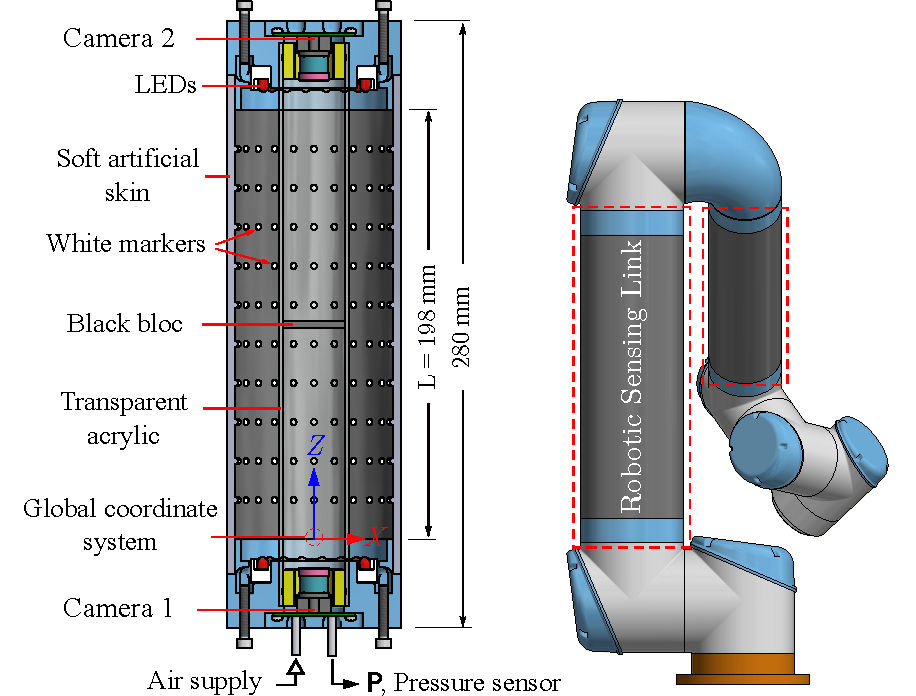
\includegraphics[width=1\columnwidth]{system_design.pdf}}
\caption{(Left) Configuration of the robot links (i.e.,  TacLINK) with large-scale tactile sensation. (Right) Sketch of a collaborative robot (UR5) equipped with TacLINK, enabling safe and intelligent interaction through the sense of touch.}
\label{fig_design}
\end{figure}
\section{System Design}
\subsection{Structure and Principle}
Figure \ref{fig_design}(a) depicts an overall view and the interior structure of TacLINK. It comprises a transparent acrylic tube that connects its two ends, acting like a bone frame for maintaining its rigidity. Each end has a connecting part that can accommodate a fisheye lens CMOS camera (ELP USBFHD01M-L21: resolution $640\times480\,\text{pixels}$, frame rate YUV2 $30\,$fps, field of view $\sim{150^{\circ}}$), and a series of high-intensity LEDs for illumination. The LED source uses a polarizing filter to produce uniform light and minimize reflected light. To block direct light from LEDs to facing camera, a black bloc is set in the middle of the acrylic tube. TacLINK is covered by soft continuous artificial skin (sensing area $\sim 49,763\,\text{mm}^2$) dyed black to completely isolate the inner space with ambient light. Based on detectability of the cameras, a total of $240$ white markers of diameter $D_\text{marker}=2.8$\,mm sit on the inner wall of artificial skin, which is firmly attached affording total sealing of the inner space between the tube and skin. An inlet supplies air to the inner space, and an outlet is connected to an external pressure sensor. Altering the inner air pressure ($0\text{--}1.5\,\text{kPa}$) inflates or deflates the skin to change its stiffness. Note that if $f$ is the focal length of a camera in pixels, and $d_{\text{min}}$ is the minimum detectable pixel size of a marker on the image, the design length of skin should satisfy $L<f\frac{D_{\text{marker}}}{d_{\text{min}}}$.


The sensing principle of TacLINK involves the two co-axial cameras, one at each end, that form a stereo camera. These cameras take consecutive pictures of markers on the inner wall of the skin, enabling the calculation of the 3-D positions of all markers on the global coordinate system. This approach took advantage of the finite element model of the skin to calculate the distribution of applied forces based on a structural stiffness matrix and extracted displacements of the markers. The contact forces can be treated as the acting concentrated force resulting from the nodal forces of the FE model.
\begin{figure}[!t]
\centering
\def\svgwidth{1\columnwidth}
\input{skin_fabrication.pdf_tex}
\caption{Casting for skin fabrication. (a) The 3-D printable parts of casting mold. (b) Filling holes of the inner mold with silicone to cast the markers. (c) Inside and top view of the actual soft skin body with distributed markers.}
\label{fig_fabrication}
\end{figure}
\subsection{Artificial Skin}
TacLINK perceives tactile information through its skin, the properties of which play an important role in sensing characteristics. In this paper, artificial skin of thickness $t=3.5\,\text{mm}$ was made of silicone rubber material Ecoflex 00-50 (Smooth-On Inc., USA) with good elasticity and relatively low mixed viscosity. The skin was fabricated by a casting method, as illustrated in Fig. \ref{fig_fabrication}. First, parts of the mold were designed by 3-D CAD software (Autodesk Inventor, Autodesk Inc., USA) and printed using a 3-D printer (M200, Zortrax S.A., Poland). The top funnel-shaped mold was customized as the pouring cup. To cast the markers, an array of hemispherical holes, of  pitches $h=18\,\text{mm}, \gamma=15^\circ$, was printed on the surface of the inner mold and filled with silicone. Second, the standard Ecoflex mixture of parts A and B (1A:1B by volume or weight) was dyed with Silc pigment before being degassed in a vacuum chamber. Using a stick, the holes on the surface of the inner mold were filled manually with white silicone (Fig. \ref{fig_fabrication}(b)). After the white markers were formed, all parts of the mold were assembled. The black silicone was poured into the inner space and allowed to cure at room temperature for about three hours. Finally, the skin body was removed manually from the casting mold. Fig. \ref{fig_fabrication}(c) shows a prototype of artificial skin with actual markers evenly distributed. 
\begin{figure}[!t]
\def\svgwidth{\columnwidth}
\input{camera_configuration.pdf_tex}
\caption{Configuration of the proposed stereo camera. We imposed that the world coordinate system (WCS) $XYZ$ located on the baseline. Its origin coincided with the center of the first end, and $X$-axis was parallel to the $X_{c_1}$- and $X_{c_2}$-axes of the camera frames $X_{c_1}Y_{c_1}Z_{c_1}$ and $X_{c_2}Y_{c_2}Z_{c_2}$. Note that the image of camera 2 was flipped over its $y_2$-axis to unify the direction of the coordinates of the two images. Thus, the image coordinates on the $x_1,x_2$- and $y_1,y_2$-axes were in the same directions as the $X$ and $Y$-axes of WCS, respectively.}
\label{fig_stereo}
\end{figure}
\section{Vision-Based Model}
This section addresses the configuration of the stereo camera, consisting of two co-axial cameras, used to produce a 3-D geometrical space. The camera was modeled by a usual pinhole, with the pixel sensors assumed to be square in shape (i.e., the focal lengths on the $x$- and $y$-axes are similar).
\subsection{Stereo Camera Model}
The objective of the vision-based system was to construct the 3-D shape of the soft skin by tracking the position of markers. Fig. \ref{fig_stereo}(a) illustrates the stereo camera consisting of two co-axial cameras with its baseline and optical axes along the centerline of the module. The $Z$-axis of the world (global) coordinate system (WCS) $XYZ$ coincided with the baseline, and its origin located at the center of the first end (with camera 1). The stereo model describes the 3-D position of a point $P=\left [X,Y,Z\right ]^\top\in \mathbb{R}^3$ in WCS captured by cameras on two image planes with corresponding 2-D points, $p=\left [x_1,y_1\right ]^\top\in \mathbb{R}^2$ , and $q=\left [x_2,y_2\right ]^\top\in \mathbb{R}^2$ (Fig. \ref{fig_stereo}(c)--(d)). Based on the geometrical relationships, the projective equation was determined to be:
\begin{align}
\begin{bmatrix} x_1 \\ y_1 \end{bmatrix} = \frac{f_1}{b_1+Z}\begin{bmatrix} X \\ Y \end{bmatrix},\;  
\begin{bmatrix} x_2 \\ y_2 \end{bmatrix} = \frac{f_2}{b_2-Z}\begin{bmatrix} X \\ Y \end{bmatrix},
\label{eq_stereo_1}
\end{align}
with 
\begin{align}
&x_1=u_1-c_{x_1},\;  y_1=v_1-c_{y_1}, \\
&x_2=u_2-c_{x_2},\;  y_2=v_2-c_{y_2}.
\end{align}
where $f_1$ and $f_2$ correspond to the focal lengths of the two cameras in pixels; $b_1$ and $b_2$ denote the position of WCS origin in two camera frames, respectively; $c_1(c_{x_1},c_{y_1})$ and $c_2(c_{x_2},c_{y_2})$ are the pixel locations of the principal points on the two pixel coordinate systems, $\set{u_1, v_1}$ and $\set{u_2, v_2}$, respectively. 

In this application, the stereo camera can be fully modelled by four intrinsic parameters $\set{f_1,f_2,c_{1},c_{2}}$ and two extrinsic parameters $\set{b_{1},b_{2}}$. The method for self-automatic calibration is presented in Section IV-D. 

The problem was to determine the 3-D location of a point through information supplied by the two cameras. For convenience, Cartesian coordinates were converted to polar and cylindrical coordinates on the image and world coordinates, respectively, where $R$ and $\varphi$ represent radial and angular coordinates of WCS (Fig. \ref{fig_stereo}(b)). Mathematically, the other form of (\ref{eq_stereo_1}) can be expressed as
\begin{equation}
\label{eq_stereo_r12}
\begin{aligned}
r_1=\frac{f_1}{b_{1}+Z}R,\quad 
r_2=\frac{f_2}{b_{2}-Z}R,
\end{aligned}
\end{equation}
where $r_1$ and $r_2$ are the radial coordinates, and the angular coordinates $\varphi_1$ and $\varphi_2$ are two arcs from $-\pi$ to $\pi$, computed from data supplied by the two cameras as (see Fig. \ref{fig_stereo}(c)--(d))
\begin{align}
&r_1 =\sqrt{x_1^{2} + y_1^{2}}, \quad \varphi_1 =\arctan2\left(y_1,x_1\right),\\
&r_2 =\sqrt{x_2^{2} + y_2^{2}},\quad \varphi_2 =\arctan2\left(y_2,x_2\right).
\end{align}
The solutions of (\ref{eq_stereo_r12}) can be derived as follows:
\begin{align}
\label{eq_stereo_Z}
&Z = \frac{f_1b_2r_2-f_2b_1r_1}{f_1r_2+f_2r_1},\\
\label{eq_stereo_R}
&R = (b_{1}+b_{2})\frac{r_1r_2}{f_1r_2+f_2r_1}.
\end{align}

Figure \ref{fig_stereo}(b)--(d) reveals that the ideal angular coordinates obey the relationship as $\varphi = \varphi_1 = \varphi_2$. In fact, the angular $\varphi_1$ and $\varphi_2$ may differ slightly, due to  misalignment of the axes of the two installed cameras. Because this discrepancy is constant, it can be corrected by compensation. The angular coordinate could be approximated as $\varphi = \frac{1}{2}(\varphi_1 + \varphi_2)$. However, because the angular coordinates discontinue at $-\pi$ and $\pi$, $\varphi$ can be calculated using the function:
\begin{equation}
\label{eq_stereo_phi}
\begin{aligned}
\varphi = 
\begin{cases} 
\frac{1}{2}(\varphi_1 + \varphi_2) & |\varphi_1 - \varphi_2|< \pi \\
\frac{1}{2}(\varphi_1 + \varphi_2)- \pi \mathrm{sign}(\varphi_1 + \varphi_2) & |\varphi_1 - \varphi_2|> \pi 
\end{cases}
\end{aligned}
\end{equation}
After $\varphi$ is obtained, $X$ and $Y$ can be calculated: 
\begin{align}
\label{eq_stereo_X}
&X = R\cos(\varphi),\\  
\label{eq_stereo_Y}
&Y = R\sin(\varphi).
\end{align}

It should be noticed that equations (\ref{eq_stereo_Z})--(\ref{eq_stereo_Y}) represent the straightforward solution of the triangulation of the stereo camera. This result enhances the ability of the proposed 3-D vision-based system to perform in real-time. 
\begin{figure}[!t]
\def\svgwidth{\columnwidth}
\input{camera_variation.pdf_tex}
\caption{Stereo variation simulation results illustrating the highest variations of error in the working space. (a) Uncertainty of $Z$ coordinate with deviations $\Delta r_1=-1/\sqrt{2}, \Delta r_2=1/\sqrt{2}$. (b) Uncertainty of radial coordinate $\Delta R$ with deviations $\Delta r_1=1/\sqrt{2}, \Delta r_2=1/\sqrt{2}$. }
\label{fig_variation}
\end{figure}
\subsection{Uncertainty of 3-D Measurement with Digital Camera}
The objective of this section is to analyze the uncertainty of stereo reconstruction, including the effects of camera parameters. This can help to optimize the best working space for design. In particular, the localization error depends on the detectability in both images associated to the projections $p(r_1,\varphi_1)$ and $q(r_2,\varphi_2)$, and is characterized by the sensitivity of imaging parameters to errors. Let $\Delta r_1$ and $\Delta r_2$ be the image plane coordinate error variables, independent from each other. Because the standard deviation of pixel error of a digital camera varies from $0$ to $1$ pixels, the normalized error variables of $\Delta r_1$ and $\Delta r_2$ are uniformly distributed within the interval of erroneously perturbed $[-1/\sqrt{2}, 1/\sqrt{2}]$\,pixels \cite{Das}. For ease of analysis, the ideal calibrated stereo parameters were assumed to be known beforehand (Table I). From (\ref{eq_stereo_Z}) and  (\ref{eq_stereo_R}), the derivative of the coordinate $Z$ and the radial coordinate $R$ with respect to $r_1$ and $r_2$, resulted in the uncertainty of ranges $Z$ and $R$ being:
\begin{align}
\label{eq_stereo_dZ}
&\Delta Z = f_1f_2\frac{b_1+b_2}{(f_1r_2+f_2r_1)^2}(r_1\Delta r_2-r_2\Delta r_1),\\
\label{eq_stereo_dR}
&\Delta R = \frac{b_{1} + b_{2}}{(f_1r_2+f_2r_1)^2}(f_1r^2_2\Delta r_1+f_2r^2_1\Delta r_2).
\end{align}
Substituting $r_1$ and $r_2$ from (\ref{eq_stereo_r12}) into (\ref{eq_stereo_dZ}) and (\ref{eq_stereo_dR}) results in the expressions of uncertainty as
\begin{align}
\label{eq_stereo_dZ2}
&\Delta Z =\frac{(b_2-Z)^2(b_1+Z)}{f_2(b_1+b_2)R}\Delta r_2-
\frac{(b_1+Z)^2(b_2-Z)}{f_1(b_1+b_2)R}\Delta r_1,\\
\label{eq_stereo_dR2}
&\Delta R = \frac{(b_1+Z)^2}{f_1(b_1+b_2)}\Delta r_1 + \frac{(b_2-Z)^2}{f_2(b_1+b_2)}\Delta r_2,
\end{align}
where $Z\in\left[0\;L\right]$, $R\in \left[R_{\text{min}}\;R_{\text{max}}\right]$ are in the working ranges.

According to (\ref{eq_stereo_dZ2}) and (\ref{eq_stereo_dR2}), the localization errors were non-linear in assessing the deviations of normalized pixel misalignments $\Delta r_1$ and $\Delta r_2$. Fig. \ref{fig_variation} shows the highest uncertainties in ranges of $\Delta Z$ and $\Delta R$ in the designed working space. The uncertainty $\Delta R$ was found to depend solely on the $Z$-coordinate, with greater certainty in the middle region ($Z \rightarrow 0.5L$, see Fig. \ref{fig_variation}(b)). Generally, markers located in the middle tend to be measured in $R$ with higher accuracy than markers near the two ends. In contrast, Fig. \ref{fig_variation}(a) indicates that the range uncertainty $\Delta Z$ increases significantly on the middle and reduces on the positive direction of $R$. Thus, markers close to the two ends and away from the centerline can be localized with higher accuracy of $Z$. In addition, increasing $f_1$ and $f_2$ can enhance precision (reduce the variations $\Delta Z$ and $\Delta R$) by installing camera with smaller pixel size, or adjusting the focal length of the lens, although the latter will reduce the view angle of the lens. 
\section{Stereo Implementation}
This section describes a robust algorithm to implement the stereo registration that unifies tracking and matching. This is followed by techniques used to measure the 3-D surface of the skin under large deformation despite occlusion or limited sight, providing the precise location of every marker.
\subsection{Configuration}
The stereo vision is designed to measure the 3-D positions of all nodes on the $24\times11$ mesh of skin (see Fig. \ref{fig_performance}(b)). Let $\ell\in \set{1,...,n_1}$ denotes the path and $\jmath\in \set{0,...,n_2}$ represents the cell, corresponding to the grid locations on the $\varphi$- and $Z$-axes, here $n_1 = 24,n_2 = 11$. The node $(\ell,\jmath)$ can be identified by labeling with an index $\ell_\jmath$ defined as (see Fig. \ref{fig_model}(a))
\begin{align}
\label{eq_stereo_16}
\ell_\jmath := n_1\times\jmath +\ell.
\end{align}
Hence, the nodes belonging to the mesh are represented by the set $\mathcal{N}=\set{\ell_\jmath}, |\mathcal{N}|=N=288$, and they were numbered from $1$ to $N$.  Herein, $\mathcal{N}$ was divide into three sets of nodes (i.e., $\mathcal{N} = \mathcal{B}_1 \cup \mathcal{M} \cup \mathcal{B}_2$): The fixed nodes were located on the two clamped edges $\mathcal{B}_1=\set{\ell_0}, |\mathcal{B}_1|=n_1$, and $\mathcal{B}_2=\set{\ell_{n_2}},|\mathcal{B}_2|=n_1$ (see Fig. \ref{fig_performance}(b)); and the free nodes or markers were tracked by cameras $\mathcal{M} = \set{\ell_\jmath}_{\jmath=1,...,n_2-1},|\mathcal{M}|=n=240$. Moreover, the full 3-D coordinates $\mathbf{X}\in \mathbb{R}^{3N}$ of all $N$-nodes was defined, with the sub-vector $\mathbf{X}_i=P(i)\in \mathbb{R}^{3}$ being the 3-D position of node $i \in \mathcal{N}$. Similarly, the sets $I_1 = \set{p(i)}$, and $I_2 = \set{q(i)}$ corresponded to the projections of all nodes on stereo images, here $ \forall i \in \mathcal{N}$, $|I_1|=|I_2|=N$.
\subsection{Non-Rigid Registration of Stereo}
Because the data obtained from image processing were the unorganized sets of 2-D points, implementation of stereo reconstruction required matching a marker's projections on the stereo images. This process is known as image registration. The earliest approaches were based on frame to frame updating \cite{Sakuma}, although this tracking method may fail under conditions of fast movement, or be affected by noise. Another approach consists of using the coherent point drift (CPD) for non-rigid registration \cite{Myronenko}; however, this iterative optimization method is rather time-consuming with large point set. To overcome these drawbacks, inspired by guidewire tracking for concentric tubes in fluoroscopic images \cite{Vandini}, this study proposes an active tracking algorithm for non-rigid point set registration of stereo.

Fig. \ref{fig_performance}(a) shows distribution of all markers in stereo images, in which each 2-D path contains $10$ makers, resulting in $24$ paths. In each image, markers appear close to each other when approaching the center, making it difficult to detect markers at the far distance. Thus, markers should be traced from the boundary area of each image to its center, corresponding to a reduction in possibility of detection. By similarity, each path can be modeled by a finite set of nodes $\vartheta_i \in \mathbb{R}^2, i = 0,1,...,n_2$, where $\vartheta_{0}$ and $\vartheta_{n_2}$ are the fixed nodes as the corresponding to the start and end points, as illustrated in Fig. \ref{fig_tracking}. Thus, assumed that under condition of deformation, the path is strongly constrained along the line $\vartheta_0\vartheta_{n_2}$, such that the constructed path connecting nodes $\set{\vartheta_i}$ should be continuous and smooth. This hypothesis is used through-out the registration algorithm.

\begin{figure}[!t]
\def\svgwidth{\columnwidth}
\input{camera_performance.pdf_tex}
\caption{A scenario for verifying the proposed stereo implementation, in which the TacLINK was in contact with a long cylindrical surface. (a) Stereo images with the proposed intuitive path tracking algorithm. (b) Reconstruction from stereo images of the 3-D deformation of artificial skin.}
\label{fig_performance}
\end{figure}
\begin{figure}[!t]
\def\svgwidth{\columnwidth}
\input{camera_tracking.pdf_tex}
\caption{The intuitive curve tracking algorithm. Using the proposed objective function with two known anchor points, $\vartheta_0$ and $\vartheta_{n_2}$, the tracking process can trace unknown nodes sequentially $\vartheta_1,\vartheta_2,...,\vartheta_{n_2-1}$.}
\label{fig_tracking}
\end{figure}

The problem of stereo registration can be formulated as seeking the optimal set of nodes for every path. Note that these 3-D paths through disparate stereo views are projected opposite on the radial direction of two image planes (see Fig. \ref{fig_performance}(a)). That is, when observed from the boundary area to the center of stereo images, the nodes on the first and second images vary  as $p(\ell_0) \to p(\ell_{n_2})$, and $q(\ell_{n_2}) \to q(\ell_{n_0})$. These curve projections of an arbitrary path $\ell$ are very constrained by two fixed nodes laid on two boundary edges (i.e., $\ell_0\in \mathcal{B}_1$ and $\ell_{n_2} \in \mathcal{B}_2$, where $\ell=1,...,n_1$ (see Fig. \ref{fig_performance}(b)).

Let $\Phi \subset \mathbb{R}^2$ denotes the generalized set of detected markers in a frame of a camera. If $\vartheta_i$ is being tracked with former tracking markers as $\vartheta_1,...,\vartheta_{i-1}$ (see Fig. \ref{fig_tracking}), then to guarantee the node $\vartheta_i$ is the node closest to node $\vartheta_{i-1}$, the closeness term for every candidate $\hat{\vartheta}_i \in \Phi$ can be calculated as
\begin{align}
\label{eq_stereo_close}
\theta^i_{\text{close}}(\hat{\vartheta}_{i},\vartheta_{i-1})=\lVert \hat{\vartheta}_{i} -\vartheta_{i-1} \rVert,
\end{align}
where $\lVert.\rVert$ denotes the standard Euclidean distance.

In contrast, when considering the smoothness of the path, it may be sufficient to characterize the curvature of the arc $\vartheta_{i-1}\hat{\vartheta}_{i}\vartheta_{n_2}$ at vertex $\hat{\vartheta}_{i}$ as $\frac{2\sin\angle \vartheta_{i-1} \hat{\vartheta}_{i} \vartheta_{n_2}}{\lVert \vartheta_{i-1}\vartheta_{n_2} \rVert}$. Based on the triangle $\triangle\vartheta_{i-1} \hat{\vartheta}_{i} \vartheta_{n_2}$ with a determined closeness term of distance $\vartheta_{i-1} \hat{\vartheta}_{i}$, then the curvature at $\hat{\vartheta}_{i}$ would depend only on the distance of $\hat{\vartheta}_{i}$ and the control line $\vartheta_{i-1} \vartheta_{n_2}$ (i.e., small deformation $\angle \vartheta_{i-1} \hat{\vartheta}_{i} \vartheta_{n_2}\approx \pi$, then $\sin\angle \vartheta_{i-1} \hat{\vartheta}_{i} \vartheta_{n_2} \propto d(\hat{\vartheta}_i,\vartheta_{i-1} \vartheta_{n_2})$). Hence, the smoothness term can be formulated as
\begin{equation}
\begin{aligned}
\label{eq_stereo_smoot}
\theta^i_{\text{smooth}}(\hat{\vartheta}_{i},\vartheta_{i-1},\vartheta_{n_2})&= d(\hat{\vartheta}_i,\vartheta_{i-1} \vartheta_{n_2})\\
&=\frac{ \lVert \vartheta_{i-1}\hat{\vartheta}_{i}\times \vartheta_{i-1}\vartheta_{n_2} \rVert}{\lVert \vartheta_{i-1}\vartheta_{n_2} \rVert}.
\end{aligned} 
\end{equation} %\bm{p}_i\bm{p}_{i-1}to simplify, 
This led to a proposed objective function to search $\vartheta_{i}$, while satisfying the criteria of closeness and smoothness. This function can be expressed as
\begin{equation}
\begin{aligned}
\label{eq_stereo_obj}
\theta^i_{\text{obj}}(\hat{\vartheta}_{i},\vartheta_{i-1},\vartheta_{n_2})&= (1-\lambda)\theta^i_{\text{close}}(\hat{\vartheta}_{i},\vartheta_{i-1}) \\&+  \lambda \theta^i_{\text{smooth}}(\hat{\vartheta}_{i},\vartheta_{i-1},\vartheta_{n_2}),
\end{aligned}
\end{equation}
where $\lambda \in [0\;1]$ is the weight that determines the relative contribution of the two factors.

In addition, obviously, not all nodes belonging to $\Phi$ are the ideal candidates for tracking $\vartheta_{i}$. For example, points $\hat{\vartheta_{i}}$, which possess the geometric relationship $\measuredangle \hat{\vartheta_{i}}\vartheta_{i-1} \vartheta_{n_2} >90^\circ$ or $\measuredangle \hat{\vartheta_{i}} \vartheta_{n_2} \vartheta_{i-1}> 90^\circ$, are unlikely to be actual marker node $\vartheta_{i}$. Thus, to ensure the reliability of the results, we created a limited search area (region of interest), constrained by two searching angles with respect to the control line $\vartheta_{i-1} \vartheta_{n_2}$ with upper limits $\alpha$ and $\beta$ shown in Fig. \ref{fig_tracking}. For this purpose, only points within region of interest were considered as candidate nodes. Therefore, for all points $\hat{\vartheta}_{i} \in \Phi$, the optimal tracking node $\vartheta_{i}$ is the node that minimizes the objective function:
\begin{align}
\label{eq_stereo_track}
&\vartheta_{i} = \underset{\hat{\vartheta}_{i} \in \Phi} {\mathrm{arg}\; \mathrm{min}} ~\theta^i_{\text{obj}}(\hat{\vartheta}_{i},\vartheta_{i-1},\vartheta_{n_2}),\\
\label{eq_stereo_roi}
&\text{subject to:} \quad \measuredangle \hat{\vartheta}_i\vartheta_{i-1}\vartheta_{n_2} <\alpha,\quad \measuredangle \hat{\vartheta}_i\vartheta_{n_2}\vartheta_{i-1} < \beta.
\end{align}
Note that (\ref{eq_stereo_roi}) is also a criterion to determine the breakpoint of a path tracking once no candidate is within a region of interest. If $\Phi_1$ and $\Phi_2$ are the sets of detected markers on stereo images after image processing at each camera frame, then the tracking process would start at the boundary area and extend to the center of the image, generating the organized sets $I_1 $ and $I_2$. This algorithm running in $\mathcal{O}(n^2)$ time is shown in Algorithm \ref{algorithm1}. 
\subsection{3-D Reconstruction}
This section presents techniques used to calculate the 3-D position of all markers based on the 2-D projections provided by the proposed registration algorithm. During physical contact, uncertainty in detection of markers may be due to a lack of sight and occlusion. Three scenarios often occur in the detection of a marker: First, the 3-D coordinates of markers captured on both cameras' images can be easily computed using (\ref{eq_stereo_Z})--(\ref{eq_stereo_Y}). Second, for markers missed or not well captured by one camera, $Z(\ell_\jmath)\approxeq \jmath\times h$ can be estimated as the initial value (which is sufficient due to the small axial $Z$-deflection of a cylinder), and the $X$- and $Y$-positions can be calculated by either camera in (\ref{eq_stereo_1}). Third, the coordinates of markers not detected on both images can be estimated by linear interpolation through its neighbors in the same path. If $\jmath^{\scriptscriptstyle -}$ and $\jmath^{\scriptscriptstyle +}$ are the nearest determined markers of the missing marker $\jmath$ on path $\ell$, where $\jmath^{\scriptscriptstyle -} < \jmath$ and $ \jmath^{\scriptscriptstyle +} > \jmath$, then the linear interpolation can be formulated as 
\begin{align}
&\mathbf{X}(\ell_\jmath)\! =w\mathbf{X}({\ell_{\jmath^{\scriptscriptstyle -}}}) + (1-w)\mathbf{X}({\ell_{\jmath^+}}),\;0<\jmath<n_2.
\end{align}
where $w = (\jmath^{{\scriptscriptstyle +}} -\jmath)/(\jmath^{\scriptscriptstyle +}-\jmath^{\scriptscriptstyle -})$ is weight function.
\begin{algorithm}[!t]
\caption{\textsc{StereoRegistration($\Phi_1,\Phi_2$)}}\label{Registration}
\textbf{Require}: Given the sets of extracted markers $\Phi_1$ and $\Phi_2$ on two images after image processing. 
%\set{p(\ell_0),p(\ell_{n_2}),q(\ell_{n_2}),q(\ell_0)}
\begin{algorithmic}[1]
\State \textbf{START} Initialize: $\alpha, \beta,$ \Comment searching angles
$\set{p(\ell_0),p(\ell_{n_2})}_{\ell=1\text{--} n_1},\set{q(\ell_{n_2}),q(\ell_0)}_{\ell=1\text{--} n_1}$  \Comment use (\ref{eq_stereo_1})
\For {$\ell \gets 1$ to $n_1$} 
\State $I_1(\ell_{0:n_2}) \leftarrow  \texttt{pTRACK}(\Phi_1,p(\ell_0),p(\ell_{n_2}),\alpha,\beta)$
\State $I_2(\ell_{n_2:0}) \leftarrow  \texttt{pTRACK}(\Phi_2,q(\ell_{n_2}),q(\ell_0),\alpha,\beta)$
\EndFor
\State \textbf{return} Organized sets $I_1$ and $I_2$\hfill
%\dashuline{
\end{algorithmic}
%\hrulefill
%\sout{\hfill}
%\hdashline\dashuline{
\textbf{function}\; {$\texttt{pTRACK}(\Phi,\vartheta_0,\vartheta_{n_2},\alpha,\beta)$} \Comment path tracking
\begin{algorithmic}[1]
\State Initialize: $\vartheta \leftarrow \set{\vartheta_0, \varnothing,...,\varnothing,\vartheta_{n_2}}$ \Comment $|\vartheta| = n_2+1$
\For {$i \gets 1$ to $n_2-1$} 
\State$\vartheta_i \leftarrow $ using (\ref{eq_stereo_track}) and (\ref{eq_stereo_roi}) 
\State \textbf{if}  $\vartheta_i = \varnothing$ \; \textbf{then} \textbf{break} \Comment breakpoint
\State  Update: $\Phi=\Phi \setminus\set{\vartheta_i}$
\EndFor\\
\Return Optimal set of nodes $\set{\vartheta_i, i = 0,...,n_2}$
\end{algorithmic}
\textbf{end function} %\operatorname{}
\label{algorithm1}
\end{algorithm}
In practice, based on the geometric constraints of 2-D paths on stereo images and stability, the tracking parameters $\alpha$ and $\beta$ equal $2\gamma= 30^\circ$ (Fig. \ref{fig_tracking}), and weight $\lambda = 0.5$ in (\ref{eq_stereo_obj}) was selected. The proposed stereo implementation worked efficiently, even in case of large deformation (e.g., Fig. \ref{fig_performance}), with the evaluation of accuracy verified in Section VII-B. However, the limitations of this system associated with elongated shape mean some markers may be occluded or overlap upon external contact e.g., multiple contacts on the same path, resulting in a 3-D reconstruction that may not well represent its actual position.
\subsection{Stereo Self-Calibration}
This vision-based sensing system requires predetermination of the parameters of the stereo camera. Although cameras can be calibrated with reference planar patterns (e.g., \cite{Zhang}), this method is unsuitable for two facing cameras due to restrictions in pattern observation. This study utilized the initial geometrical position of markers in known positions to determine the stereo parameters with self-calibration ability to enable automatic calibration. In this scenario, $(R_{0i},\varphi_{0i},Z_{0i}), \forall i \in \mathcal{M}$ were regarded as a set of markers at their initial state and $(r_{1i},\varphi_{1i})$ and $(r_{2i},\varphi_{2i})$ as its measured projections. 
\subsubsection{Estimation of Camera Parameters}
%as in \cite{Tsai}, 
Geometrically, due to the symmetric distribution of 3-D markers around the $Z$-axis, the projections of markers on each image plane should be symmetric relative to the origin of its coordinates. Therefore, the principal points $c_1$ and $c_2$ can be simply determined by computing the mean centroids of all markers in pixel coordinates as $c_{x_1} = \frac{1}{n}\sum\nolimits_{i}u_{1i},\: c_{y_1} = \frac{1}{n}\sum\nolimits_{i}v_{1i}$, and $c_{x_2} = \frac{1}{n}\sum\nolimits_{i}u_{2i},\:c_{y_2} = \frac{1}{n}\sum\nolimits_{i}v_{2i}$, where $\forall i \in \mathcal{M}$, $n=240$ represents the entire set of markers. For ease of implementation, after retrieving the principal points, a center square of area $S\times{S}\,\text{pixels}^2$ around each principal point was cropped to yield a uniform image size before image processing, here $S=400\,\text{pixels}$. The principal points were redefined as $(\frac{S}{2},\frac{S}{2})$, and the calibration objective was to determine the primary stereo parameters $\bm{\mathcal{C}}=[f_1, f_2, b_1, b_2]^{\top}$. 
From the projective relationship (\ref{eq_stereo_r12}), the stereo parameters can be determined by minimizing the cost function:
\begin{equation}
\begin{aligned}
\label{eq_stereo_cali}
\min_{\bm{\mathcal{C}}} \;\sum_{i\in \mathcal{M}} (&\lVert R_{0i}f_1-r_{1i}b_1 - r_{1i}Z_{0i} \rVert^2\\ 
&+ \lVert R_{0i}f_2-r_{2i}b_2 + r_{2i}Z_{0i} \rVert^2).
\end{aligned}
\end{equation}

Note that (\ref{eq_stereo_cali}) requires at least two reference points to derive four unknown parameters $\bm{\mathcal{C}}$. This minimization problem, a linear least-squares $\min_{\bm{\mathcal{C}}}\lVert\bm{A}\bm{\mathcal{C}}-\bm{b}\rVert^2$, can be solved with MATLAB's built-in $\mathrm{mldivide}$ function i.e., $\bm{\mathcal{C}}=\mathrm{mldivide}(\bm{A},\bm{b})$.
\begin{table*}[!t]
\centering
\renewcommand{\arraystretch}{1.1} 
\caption{Self-Calibration Results of Stereo Camera Parameters $(\mu \pm  \sigma)$}
\setlength{\tabcolsep}{3pt}
\begin{tabular}{p{0.1\linewidth}p{0.1\linewidth}p{0.1\linewidth}p{0.1\linewidth}p{0.1\linewidth}p{0.1\linewidth}p{0.1\linewidth}}
\toprule
\hfil Camera $i$&  \hfil $f_{i}\: [\text{pixels}]$ & \hfil $b_{i}\: [\text{mm}]$ & \hfil $c_{xi}\: [\text{pixels}]$ & \hfil $c_{yi}\: [\text{pixels}]$& \hfil $k_{1i}\:[\times 10^{-7}]$& \hfil $k_{2i}\:[\times 10^{-11}]$\\
\midrule
\hfil $1$ &     \hfil $226.91\pm 0.09$ & \hfil $26.50\pm 0.04$ & \hfil $322.76\pm 0.01$ & \hfil $225.23\pm 0.01$& \hfil $27.85\pm 0.09$& \hfil $-14.09\pm 0.04$\\
\hfil $2$ &    \hfil $226.54\pm 0.06$ & \hfil $226.49\pm 0.02$ & \hfil $299.70\pm 0.00$ & \hfil $251.89\pm 0.01$& \hfil $21.08\pm 0.10$& \hfil $-11.58\pm 0.05$\\
\bottomrule
%\multicolumn{3}{l}{Subscript $(.)$ corresponds to the camera index.}
\end{tabular}
\label{table_stereo}
\end{table*}
\subsubsection{Correction of Lens Distortion}
When using wide angle lenses, it is necessary to consider the lens distortion of camera. In this camera configuration, we only assessed the term for radial distortion. If $\breve{r}_1$ and $\breve{r}_2$ are the actual observed coordinates, and $r_1$ and $r_2$ are the ideal radial image coordinates according to the pinhole model described in (\ref{eq_stereo_r12}) and (\ref{eq_stereo_cali}), then the radial division distortion model \cite{Fitzgibbon} can be written as
\begin{align}
\label{eq_stereo_r1}
&r_1=\frac{\breve{r}_1}{1+k_{11}\breve{r}_1^2 +k_{21}\breve{r}_1^4 },\\ 
\label{eq_stereo_r2}
&r_2=\frac{\breve{r}_2}{1+k_{12}\breve{r}_2^2 +k_{22}\breve{r}_2^4},
\end{align}
where $\set{k_{11}, k_{21}}$ and $\set{k_{12}, k_{22}}$ are the coefficients of the radial distortion of the two camera lenses, respectively.  

To determine the distorted coefficients, the preliminary parameters $\bm{\mathcal{C}}$ in (\ref{eq_stereo_cali}) were estimated by ignoring distortion. Then, the ideal image coordinates $r_1$ and $r_2$ were determined using the equations in (\ref{eq_stereo_r12}). Thus, from (\ref{eq_stereo_r1}) and (\ref{eq_stereo_r2}), the coefficients $\bm{\mathcal{L}}=[k_{11},k_{21},k_{12},k_{22}]^{\top}$ can be estimated by minimizing the cost function as
\begin{equation}
\begin{aligned}
\label{eq_stereo_dis}
\min_{\bm{\mathcal{L}}} \;\sum_{i\in \mathcal{M}}&(\lVert r_{1i}\breve{r}_{1i}^2k_{11} + r_{1i}\breve{r}_{1i}^4k_{21} +(r_{1i}- \breve{r}_{1i}) \rVert^2 \\&+\lVert r_{2i}\breve{r}_{2i}^2k_{12} + r_{2i}\breve{r}_{2i}^4k_{22} +(r_{2i}- \breve{r}_{2i}) \rVert^2).
\end{aligned}
\end{equation}%\nonumber

Once $\bm{\mathcal{L}}$ is obtained, the parameters $\bm{\mathcal{C}}$ can be recomputed by recalling (\ref{eq_stereo_cali}), with this procedure repeated until reaching convergence. The root-mean-square error (RMSE) of coordinates was used to assess the calibration process, as shown in Fig. \ref{fig_iteration}. This figure shows rapids convergence of calibrated coordinates RMSE within fewer than four iterations and a significant reduction in erroneous results. 
\begin{figure}[!t]
\def\svgwidth{\columnwidth}
\input{camera_iteration.pdf_tex}
\caption{Calibration results for each iteration: RMSE of  coordinates for estimating stereo parameters and lens distortion.}
\label{fig_iteration}
\end{figure}
\begin{figure}[!t]
\def\svgwidth{\columnwidth}
\input{camera_calibration.pdf_tex}
\caption{Illustration of the initial 3-D position of markers (roundly marked) using the calibrated parameters.}
\label{fig_calib3D}
\end{figure}
The calibration process was performed a total of 20 times, yielding the camera parameters and distortion coefficients shown in Table I. These results were used to verify some parameters of the stereo camera configuration. For example, the length of artificial skin after calibration can be calculated as $L=b_2-b_1 \approx \text{200.0\,mm}$ (see Fig. \ref{fig_stereo}), while the designed value is $198.0$\,mm (see Fig. \ref{fig_design}), i.e., the absolute was $2.0$\,mm, or $1.01\%$. With calibrated parameters, Fig. \ref{fig_calib3D} illustrates the initial geometric 3-D paths of markers and their measured locations. The average RMSE of the calibrated coordinates $R$, $Z$ and 3-D were $0.58\,\text{mm}$, $0.55\,\text{mm}$ and $0.80\,\text{mm}$, respectively.

By referring to the pattern of markers, we could determine the intrinsic and extrinsic parameters of the stereo camera and lens distortion. Note that although light traveling through the acrylic tube would be refracted (incident and refracted rays are shifted), the system’s calibration used refracted images, resulting in the parameters of lens distortion covered this effect.
\section{FE Model of Artificial Skin}
This section introduces the finite element model of the skin to establish the relationship between nodal displacements of the markers and external forces. For ease of modeling, the skin was assumed to be linearly elastic. The skin was modeled by the flat shell elements combining membrane and bending behaviors based on Reissner-Mindlin theory \cite{Onate}. Only the static model was considered, ignoring the gravitational effect on the skin, as we hypothesized that the effect of gravity on the skin was much smaller than the effects of the range of measured forces.
\subsection{Meshing and Geometry of the Element}
Owing to its 3-D symmetric shape, the skin can be equally discretized into a mesh of $N_{\text{e}}=264$ elements (Fig. \ref{fig_model}(a)). The rectangular domain $\Omega$ of a shell element is estimated as $2a = h$ and $2b = 2R_0\sin\left (\gamma/2\right )$ (Fig. \ref{fig_model}(c)). To build the elemental and global vectors and matrices, it was necessary to define mesh topology providing a crucial nodal connectivity of elements. By positioning an element $e \in \set{1,...,N_{\text{e}}}$ by the node associated with the left bottom corner (Fig. \ref{fig_model}(b)). The element at $(\ell,\jmath)$ is numbered $e=\ell_\jmath$ (\ref{eq_stereo_16}) and formed by four nodes distributed counter-clockwise, $\hat{1}(\ell,\jmath+1)$, $\hat{2}(\ell,\jmath)$, $\hat{3}(\ell+1,\jmath)$, and $\hat{4}(\ell+1,\jmath+1)$,  where $\jmath = 0,...,n_2, \ell = 1,...,n_1-1$; if $\ell=n_1$, then nodes 3 and 4 are $\hat{3}(1,\jmath)$ and $\hat{4}(1,\jmath+1)$, respectively. Fig. \ref{fig_model}(a) shows the FE mesh of the skin with node and element numbering.

For ease of computation, the displacement field of each element should be described in its local domain. In this paper, besides the global coordinate system, the four-node shell element was formulated in the local coordinates $\set{\hat{x},\hat{y},\hat{z}}$, and the natural coordinates $\set{\xi,\eta}$ shown in Fig. \ref{fig_model}(c). If the $\hat{x}$-axis is defined as the opposite of the $Z$-axis, and the edge 2-3 defines the $\hat{y}$-direction, then the $\hat{z}$-axis is obtained by the cross product of $\hat{x}$- and $\hat{y}$-axes. Each  shell element node has five degrees of freedom i.e., in-plane displacements $u_{\hat{x}},u_{\hat{y}}$, lateral displacement $u_{\hat{z}}$, and rotations $\theta_{\hat{x}}$ and $\theta_{\hat{y}}$ of $\hat{z}$-axis in the planes $\hat{x}\hat{z}$ and $\hat{y}\hat{z}$, respectively \cite{Onate}. 
\subsection{FE Equations and Simulation}
The state equation of an element in static equilibrium can be determined from its local domain (Fig. \ref{fig_model}(c)) by applying the principle of virtual work (PVW) as (see Table II and Appendix for a detailed explanation and derivation of variables)  
\begin{align}
\label{eq_fem_pvw}
\underbrace{\int_{\Omega}\delta\hat{\bm{\epsilon}}^{\top} \hat{\bm{\sigma}}\;\mathrm{d}\Omega}_{\text{Internal virtual strain energy}} = \underbrace{\int_{\Omega} \delta \hat{\mathbf{u}}^{\top} \hat{\mathbf{s}} \, \mathrm{d}\Omega+ \delta \hat{\mathbf{d}}^{\top} \hat{\mathbf{f}}^{\text{ext}}}_{\text{External virtual work}}.
\end{align}
The element equation in equilibrium can be expressed as
\begin{equation}
\label{eq_fem_localeq}
\begin{aligned}
\hat{\mathbf{k}}\hat{\mathbf{d}} = \hat{\mathbf{f}}_{\text{pressured}} + \hat{\mathbf{f}}^{\text{ext}}.
\end{aligned}
\end{equation}

The element equation (\ref{eq_fem_localeq}) represents the relationship between nodal displacements $\hat{\mathbf{d}}$, the distributed force $\hat{\mathbf{f}}_{\text{pressured}}$ due to inner air pressure $\mathsf{P}$ (\ref{eq_fem_pressured}), and the external concentrated force $\hat{\mathbf{f}}^{\text{ext}}$.
These elements locate on different local orientations, thus, to build the global equation, the element equation (\ref{eq_fem_localeq}) must be expressed in the global coordinates as
\begin{align}
\label{eq_fem_globaleq}
\mathbf{k}\mathbf{d} = \mathbf{f}_{\text{pressured}} +\mathbf{f}^{\text{ext}}.
\end{align}
where details of its derivation can be found in Appendix.

\begin{figure}[!t]
\def\svgwidth{1\columnwidth}
\input{fem_model.pdf_tex}
\caption{Three-dimensional FE model for artificial skin. (a) Finite element mesh of $N_{\text{e}}=264$ elements and $N=288$ nodes. (b) Mesh topology. (c) Geometry of a rectangular flat shell element.}
\label{fig_model}
\end{figure}
\begin{table}[htp]
\centering
\renewcommand{\arraystretch}{1} 
\caption{Nomenclature for Section V and VI}
\setlength{\tabcolsep}{3pt}
\begin{tabular}{P{30pt}p{200pt}}
\toprule
%Symbol&   \makecell{Description} \\ 
\textbf{Symbol}& \textbf{Description} \\ 
\midrule
$\hat{\mathbf{u}}$& Displacement field vector, $= [u_{\hat{x}}\;u_{\hat{y}}\;u_{\hat{z}}\;\theta_{\hat{x}}\;\theta_{\hat{y}}]^{\top}$. \\
$\hat{\mathbf{s}}$& Surface load of inner air pressure $\mathsf{P}$, $= [0\;0\;\mathsf{P}\;0\;0]^{\top}$. \\
$\hat{\bm{\epsilon}}$&$\in \mathbb {R}^{8}$ Strain vector.\\
$\hat{\bm{\sigma}}$& $\in \mathbb {R}^{8}$ Stress vector.\\
$\hat{\mathbf{k}}, \mathbf{k}$&  $\in \mathbb {R}^{20 \times20}, \in \mathbb {R}^{24 \times24}$ Element stiffness matrices.\\
\hdashline
\makecell[c]{$\hat{\mathbf{d}}, \mathbf{d}$\\\\\hfill}& \makecell[l]{$\in \mathbb {R}^{20},\in \mathbb {R}^{24}$ Nodal displacement vectors of an element,\\ $\hat{\mathbf{d}}_i= [u_{\hat{x}_i}\;
u_{\hat{y}_i}\;u_{\hat{z}_i}\;\theta_{\hat{x}_i}\;\theta_{\hat{y}_i}]^{\top}, i=1\text{--}4$,\\ $\mathbf{d}_i= [u_{X_i}\;
u_{Y_i}\;u_{Z_i}\;\theta_{X_i}\;\theta_{Y_i},\theta_{Z_i}]^{\top}, i=1\text{--}4$.}\\
\hdashline
\makecell[c]{$\hat{\mathbf{f}},\mathbf{f}$\\\\\hfill}& 
\makecell[l]{$\in \mathbb {R}^{20}, \in \mathbb {R}^{24}$ Nodal force vectors of an element, \\$\hat{\mathbf{f}}_i= [f_{\hat{x}_i}\;
f_{\hat{y}_i}\;f_{\hat{z}_i}\;m_{\hat{x}_i}\;m_{\hat{y}_i}]^{\top}, i=1\text{--}4,$\\
$\mathbf{f}_i= [f_{X_i}\; 
f_{Y_i}\;f_{Z_i}\;m_{X_i}\;m_{Y_i}\,m_{Z_i}]^{\top},  i=1\text{--}4$.}\\
\hdashline
$\mathbf{K}$& $\in \mathbb {R}^{6N \times 6N}$  Global stiffness matrix.\\
\hdashline
\makecell[c]{$\mathbf{D}$\\\hfill}& 
\makecell[l]{$\in \mathbb {R}^{6N}$ Global displacement vector, \\
$\mathbf{D}_i= [u_{X_i}\; 
u_{Y_i}\;u_{Z_i}\;\theta_{X_i}\;\theta_{Y_i}\,\theta_{Z_i}]^{\top},  i=1\text{--}N$.}\\
\hdashline
\makecell[c]{$\mathbf{F}$\\\hfill}& 
\makecell[l]{$\in \mathbb {R}^{6N}$ Global force vector, \\
$\mathbf{F}_i= [F_{X_i}\; 
F_{Y_i}\;F_{Z_i}\;M_{X_i}\;M_{Y_i}\,M_{Z_i}]^{\top},  i=1\text{--}N$.}\\
%\hline
\bottomrule
\multicolumn{2}{l}{Overscript\, $\hat{}$\, indicates variables expressed in the local coordinates $\hat{x}$, $\hat{y}$, and $\hat{z}$.}\\
\multicolumn{2}{l}{All quantities are presented in SI units.}
\end{tabular}
\label{table3}
\end{table}
Finally, the system equation of the FE model is established by assembling together all (\ref{eq_fem_globaleq}) of elements $e=1,2,...,N_{\text{e}}$ based on the connected nodes in the meshing topology as
\begin{equation}
\label{eq_fem_equation}
\begin{aligned}
\mathbf{K}\mathbf{D}= \mathbf{F}_{\text{pressured}}+\mathbf{F}^{\text{ext}}.
\end{aligned}
\end{equation}

Besides, as the skin of the TacLINK is clamped at both ends, with the degrees of freedom of all nodes set at zero, then the boundary conditions of the FE equation (\ref{eq_fem_equation}) are expressed as
\begin{equation}
\label{eq_fem_boundary}
\begin{aligned}
\mathbf{D}_{i} = \bm{0},\; \forall i\in \mathcal{B}_1\cup \mathcal{B}_2.
\end{aligned}
\end{equation}
To verify the ability of the FE model to describe the physical characteristics of the skin, the model was built numerically and implemented in MATLAB. Young's modulus $E$ of silicone material was calibrated to be $0.1$\,MPa (see Section VII-C) and Poison's ratio $\nu$ was set as $0.5$. TacLINK was successfully simulated under multiple contacts at different locations with varied pressure. The displacement vector $\mathbf{D}$ in  (\ref{eq_fem_equation}) was found to be solvable with the boundary conditions (\ref{eq_fem_boundary}), as indicated in \cite{Young}. Fig. \ref{fig_simulation} shows results of subjecting the TacLINK to a normal force $0.2$\,N at node \#$127(7,5)$ (Fig. \ref{fig_simulation}(a)), and with the application of additional inner pressure of $0.5$\,kPa (Fig. \ref{fig_simulation}(b)). These findings indicate that the FE model can provide a realistic response of the skin, including 3-D deformation, stress-strain, and reaction force at fixed ends. Based on this model, we can evaluate the overall stiffness of the skin to optimize the design and choose suitable skin material for particular applications.
%\pagebreak
\section{FE Model-based Tactile Force Sensing}
Tactile force $\mathbf{F}^{\text{tac}}$ can be defined as the external force $\mathbf{F}^{\text{ext}}$ acting on the skin surface, excluding the distributed forces generated by inner pressure $\mathbf{F}_{\text{pressured}}$. Based on (\ref{eq_fem_equation}), we could derive a straightforward relationship as
\begin{equation}
\label{eq_fem_force}
\begin{aligned}
\mathbf{F}^{\text{tac}}=\mathbf{K}\mathbf{D}_{\text{measured}}-\mathbf{F}_{\text{pressured}}.
\end{aligned}
\end{equation}
The scope of this paper considers only the measured translations $(u_{X},u_{Y},u_{Z})$ with forces $(F_{X},F_{Y},F_{Z})$, ignoring the degrees of freedom of nodal rotations and moments. Thus, the measured nodal displacement vector $\mathbf{D}_{\text{measured}}$ can be computed from the output vector $\mathbf{X}$ of the stereo camera as
\begin{align}
\label{eq_fem_dis}
\mathbf{D}_{\text{measured},i}:= \left [\right.\Delta{\mathbf{X}}_i^\top\quad\underbrace{0\quad0\quad0}_{\text{rotations}}
\left .\right ]^\top, \;\forall i \in \mathcal{N}.
\end{align}
where $\Delta{\mathbf{X}} = {\mathbf{X}}-\mathbf{x}$, and $\mathbf{x}$ is the coordinates vector of nodes in the undeformed state of artificial skin.  

The computed tactile force vector $\mathbf{F}^{\text{tac}}$ is based on sampling a large number of points i.e., $N=288$ nodes with $3\times{N}$ force components. In practice, errors during 3-D reconstruction induce errors in force calculations. Based on cylindrically shaped skin, we simulated evaluation of this effect in the tangential, axial and radial directions. For ease of analysis, we assumed that $\delta_{\text{err}}\,$mm was the absolute error in every direction. Node \#127 (see Fig. \ref{fig_simulation}) was chosen and constrained in the tangential ($X$-axis), radial ($Y$-axis) and axial ($Z$-axis) deflections as $\mathbf{D}_{127} = \left [\delta_{\text{err}},\delta_{\text{err}},\delta_{\text{err}},0,0,0\right]^\top$. Solving with (\ref{eq_fem_equation}) and (\ref{eq_fem_boundary}), we calculated the reaction force at node \#127 as  $\mathbf{F}^{\text{ext}}_{127} = \left [0.08\delta_{\text{err}},0.02\delta_{\text{err}},0.30\delta_{\text{err}},0,0,0\right]^\top$. These findings indicated that spatial errors result in much higher errors of force in the tangential ($\sim{4}\,$ times) and axial ($\sim{15}\,$ times) directions than in the radial direction. Under conditions of normal contact with the cylindrical skin surface, the radial displacements should be greater than displacements in other directions. Thus, to ensure the reliability of each nodal force, only the radial component was considered as
\begin{align}
\label{eq_fem_nforce}
F_R= F_X\cos\varphi + F_Y\sin\varphi.
\end{align}
Also, for practical reasons, we only considered the computed force $F_R$ above a certain threshold i.e., $f_\text{thresh}= 0.02\delta_{\text{err}}$\,N. Finally, the tactile forces were regarded as the concentrated forces acting at free nodes $\mathbf{F}^{\text{tac}}_i,\forall i \in \mathcal{M}$, and as the reaction forces acting at two edges $\mathbf{F}^{\text{tac}}_i,\forall i \in \mathcal{B}_1 \cup \mathcal{B}_2$.
\begin{figure}[!t]
\def\svgwidth{\columnwidth}
\input{fem_simulation.pdf_tex}
\caption{FE model simulation results for soft artificial skin. (a) Skin deformation by a normal force $0.2$\,N at node \#127(7,5). (b) Response of skin to additional inner air pressure $\mathsf{P}=0.5$\,kPa.}
\label{fig_simulation}
\end{figure}
\section{Experimental Validation}
\subsection{Experimental Platform}
The experimental platform set up to calibrate and evaluate the operation of the TacLINK is shown in Fig. \ref{fig_experiment}. Within the platform, TacLINK is fixed in a rigid vertical position. The inner pressure was adjusted using a pneumatic throttle valve, and measured with a pressure sensor (MPXV7007, NXP Inc., USA) through a 16-bit ADC data acquisition board (USB-231, Measurement Computing Corp., USA), with a measurement resolution of pressure of $0.85$\,Pa. To provide precise displacement of external contact with the skin, we set up a 6-DOF robotic arm (VP-6242, Denso Robotics, Japan) which can precisely displace with high repeatability of $\pm0.02\,\text{mm}$. A probe was attached to the center of the robot's end-effector through a 3-axes force sensor (USL06-H5-50N, Tec Gihan, Japan). 
The robot moved the probe in plane $OYZ$ and pushed it horizontally against the skin at different nodes on the seventh path ($\ell=7$). To accurately push the entire cross-sectional area of the marker, we utilized a cylindrical probe as a standard screw M3 with a larger diameter $D_{\text{probe}}=5.5$\,mm. 

The experiment was run on a desktop PC with an i7-7700 processor at 3.60\,GHz and 8\,GB of RAM. The system performed in real-time at about 13\,Hz, with time to capture stereo pictures $\sim{0.003}$\,s, image-processing $\sim{0.025}$\,s, stereo registration $\sim{0.037}$\,s, and both 3-D shape and force reconstruction completed within $0.0002$\,s, with MATLAB code.
\subsection{Assessment of the Accuracy of 3-D Reconstruction} 
The performance of stereo-based 3-D reconstruction was verified by evaluating the measurement error of radial displacement of free nodes on a path. Radial direction was found to play the most important role (see Section VI), and it was challenging to determine the true value of $Z$-deflection. Specifically, the robot arm was controlled, allowing the probe to create radial displacements $\Delta{R}$ of $-5$ and $-10$\,mm every ten nodes on the seventh path (Fig. \ref{fig_experiment}). Ten trials were performed at an inner air pressure of zero. Fig. \ref{fig_accurancy} shows the measured radial deflections of ten cells $\jmath=1,2,...,10$ compared with baseline robot motion $\Delta{R}$. Because of geometric constraints on the skin, two nodes located near two ends $\jmath=1,10$ could only be displaced by $-5$\,mm. The experiment results of this testing showed that the absolute errors were below $0.7$\,mm, corresponding to a full-scale error $\sim{5}\%\,$FS (with FS $15$\,mm). This error may also derive from several parts of the system (e.g., poor fabrication and installation tolerances with soft materials). These findings indicate that the proposed vision system is both efficient (see Fig. \ref{fig_performance}) and accurate in estimating deformation of the 3-D skin. 
\subsection{Young's Modulus Calibration}
The elastic Young's modulus $E$ of the skin material was estimated from a compression test performed under quasi-static conditions. Air was provided at different levels of pressure $\mathsf{P} \in \mathcal{P}=\set{0.5, 1.0, 1.5}\,\text{kPa}$ for a total of 30 trials. During inflation, a program automatically recorded data at these pressures, enabling estimation of parameter $E$ by minimizing the difference between experimentally determined deformation and deformation predicted by the linear FE model as
\begin{align}
\label{eq_experiment_calib}
&\min_E \quad \left(\sum\nolimits_{\mathsf{P}\in \mathcal{P}} \lVert \mathbf{D}_\text{measured} -\frac{E^{*}}{E} \mathbf{D}_\text{FEM*} \rVert^2 \right)\\
&\text{s.t.} \quad E = E^{*}\frac{\sum_{\mathsf{P}\in \mathcal{P}}  \lVert  \mathbf{D}_{\text{FEM*}} \rVert^2}{\sum_{\mathsf{P} \in \mathcal{P}}  {\mathbf{D}_\text{measured} \cdot\mathbf{D}_\text{FEM*}} }
\label{eq_experiment_E}
\end{align}
where $\mathbf{D}_\text{measured}$ and $\mathbf{D}_\text{FEM*}$ are the nodal displacement vectors obtained from  experimental data and the FE model (with assigned Young's modulus $E^{*}=1$\,MPa), respectively. 

Because the sum of the squares errors in (\ref{eq_experiment_calib}) is a quadratic function of $\frac{1}{E}$, $E$ can be easily derived as in (\ref{eq_experiment_E}). 
Based on the symmetric shape of the FE model under pressure (i.e., similar curvature of every path), the experimentally determined displacement of all paths was averaged to calculate (\ref{eq_experiment_E}) on a path. Fig. \ref{fig_calibration} shows the experimental displacements for ten nodes on a path along the skin, together with the theoretical curvature (lines) of the FE model in response to varying levels of inner pressure. The experimental data fit those of the FE model well with an estimated $E$ value of $0.1\,\text{MPa}$ and an average RMSE for nodal displacements of $0.38\,\text{mm}$.
\begin{figure}[!t]
\def\svgwidth{1\columnwidth}
\input{experiment_setup.pdf_tex}
\caption{The experimental platform with all related equipment for measurement. A robot arm was equipped to push the elastic skin through a probe attached to the end-effector through a 3-axes force sensor.}
\label{fig_experiment}
\end{figure}
\begin{figure}[!t]
\def\svgwidth{1\columnwidth}
\input{experiment_accurancy.pdf_tex}
\caption{Measured displacements of ten nodes on a path were compared with true deflections created by robot motion.}
\label{fig_accurancy}
\end{figure}
\begin{figure}[!t]
\def\svgwidth{1\columnwidth}
\input{experiment_inflation.pdf_tex}
\caption{Comparison of experimental data (solids) and calibrated FE model (lines) of skin curvature in response to applied inner pressures of $0.5,1,$ and $1.5$\,kPa, estimating Young's modulus of the silicone material (Ecoflex 00-50).}
\label{fig_calibration}
\end{figure} 
\subsection{Evaluation of FE Model-based Tactile Force Sensing}
\subsubsection{Single-Point Contact}
The finite element model of the skin (\ref{eq_fem_equation}) enables TacLINK to estimate the external acting force distribution on the whole skin body (\ref{eq_fem_force}) (i.e., $\mathbf{F}^{\text{tac}}_{i}, \forall i\in \mathcal{M}$).
This experiment  evaluated the tactile force-sensing ability and assessed the characteristics of TacLINK when interacting at a single point under varying inner air pressures. The robot arm was manipulated so that the probe pushing the skin at node \#127 along the Y-axis (see Fig. \ref{fig_experiment}) created two desired radial displacements $\Delta{R} \in \set{-5, -10}$\,mm in different conditions of inner air pressure $\mathsf{P} \in \set{0, 0.5, 1.0,1.5}$\,kPa for ten trials. Note that although the ideal probe should be narrow enough to represent a point load, a small probe may cause undesired deformation in the thickness direction at the contact point. To mitigate these issues, a cylindrical probe of diameter $D_{\text{probe}}=5.5$\,mm was employed. The tactile force of TacLINK was also simulated by setting an additional boundary condition for (\ref{eq_fem_equation}) on the $Y$-axis as $\mathbf{D}_{127,Y} = \Delta{R}$. Fig. \ref{fig_exp_force} shows the comparison between the probe force and the tactile forces at node \#127 obtained from TacLINK ($\mathbf{F}^{\text{tac}}_{127}$) and simulation ($\mathbf{F}^{\text{ext}}_{127}$) at each level of deflection $\Delta{R}$ and inner air pressure $\mathsf{P}$.

In the absence of inner pressure ($0$\,kPa), the resultant forces matched well at every deflection. However, when pressure was applied, the nodal tactile force of TacLINK increased linearly but was significantly lower than the probe force. This difference may be due to the probe not being small enough to represent an ideal point load contact scenario in simulation (see Fig. \ref{fig_exp_force}). The inner air pressure acting on the inner side of the skin gave rise to tension stresses (circumferential $\sigma_{\hat{y}}$ and longitudinal $\sigma_{\hat{x}}$ stresses, see Fig. \ref{fig_model}(c)) in its wall, resulting in a highly increased probe force to move the probe with contact area $S_{\text{probe}}=\frac{\pi}{4}{D^2_\text{probe}}= 23.8\,\text{mm}^2$ that caused greater deformed contact area surrounding the assigned node. The mesh size ($2a=18\,\text{mm}, 2b=9.5\,\text{mm}$) was not dense enough to describe actual deformation in the contact area caused by the probe. The computed tactile force distribution of TacLINK representing the probe force would also be distributed on the adjacent nodes, and the largest nodal tactile force should be at node \#127 shown in Fig. \ref{fig_reconstruction}(a). Consequently, single point force contact scenario using a probe attached in a loadcell is rather challenging (i.e., create an ideal point load and perceive the entire applied force by a nodal tactile force), because the probe has a finite area and the skin is soft, etc. The obtained results indicate that TacLINK is capable of determining the distribution of applied forces.

Varying the probe forces revealed actual reaction of artificial skin e.g., the maximum probe forces per unit area ($\equiv\frac{F_{\text{probe}}}{S_{\text{probe}}}$) at $0\,\text{kPa}$ and $1.5\,\text{kPa}$ were $0.84\,\text{N}/\text{cm}^2$ and $5.6\,\text{N}/\text{cm}^2$, respectively. As the inner pressure increased, so did the slope of probe force, thus by controlling the inner pressure we could alter remarkably the nominal stiffness of the skin and change the interactive interface of TacLINK. 
\subsubsection{Multiple Large-Areas Contact}
Because the aim of TacLINK is to sense contacts with humans, we performed an experiment in which a human used two fingers to randomly touch different areas of the artificial skin. Fig. \ref{fig_reconstruction}(b) shows the robust reconstruction of both 3-D deformation and external acting forces in large and multi-contact regions. Tactile forces were distributed only in contact regions; but were absent from other regions, even those that showed deformation. Generally, under conditions of physical interaction in any position, TacLINK registers detailed 3-D deformation of the skin surface caused by external forces, the location and intensity of which are determined by tactile force distribution. It is noteworthy that previous vision-based tactile force techniques with markers, such as machine learning \cite{Yuan}, and experimental calibration \cite{Sato}, \cite{Ito}, could estimate the total force applied not determine the distribution of applied forces in scenarios such as under large area or multiple point contacts. Also, tactile skin designs with discrete sensing elements \cite{Schmitz}, \cite{Philipp} cannot detect touch in areas not occupied by such elements, however, using the FEM to reconstruct forces over a continuous area, the proposed sensing system can simultaneously perceive tactile forces throughout the skin surface (see supplementary video).
\begin{figure}[!t]
\def\svgwidth{1\columnwidth}
\input{experiment_force.pdf_tex}
\caption{Probe forces applied yielding radial deflections $\Delta{R}$ at node \#127 compared with the nodal tactile forces at node \#127 obtained from TacLINK and simulation under different inner air pressures.}
\label{fig_exp_force}
\end{figure}
\begin{figure}[!t]
\def\svgwidth{1\columnwidth}
\input{force_resconstruction.pdf_tex}
\caption{Experimental results of tactile force reconstruction on the three-dimensional body of the skin surface. (a) Test with single-point (node) contact at node \#127. (b) Performance with multiple large-area contacts.}
\label{fig_reconstruction}
\end{figure}
\section{Discussion}
\subsection{Limitations}
Using only two co-axial cameras on a simple structure, the proposed system using FEM can efficiently construct the distribution of forces acting on the elongated surface of soft artificial skin. However, during tracking the skin surface,  presence of reflected bright regions or occlusion due to multiple contacts on the same path, may impede image processing and affect the performance of the visual-based system. Since FEM was originally formulated based on the principle of virtual work in elasticity (\ref{eq_fem_pvw}), the performance of force computation highly depends on the element model (strains $\hat{\bm{\epsilon}}$ and stresses $\hat{\bm{\sigma}}$) and mesh size ($2a,2b$) representing the strain energy of actual skin deformation (especially in contact regions). Thus, in this paper, force reconstruction might not well represent force intensity, especially over large contact areas with inner air pressure applied. Further design improvements and investigations are needed to overcome these limitations.
\subsection{Technical Issues}
The structural rigidity of TacLINK is ensured by a hollow tube with transparent acrylic materials. Although its working load limit can be reduced compared with metals, we can determine suitable dimensions of the tube for specific applications. If  $M_d$ is the working load design moment (combined bending and torsion), and $[\sigma]$ represents permissible stress, then the strength condition to choose inner $d$ and outer $D$ diameters of the tube can be expressed as \cite{Belyaev} 
\begin{equation}
%\label{eq_45}
\begin{aligned} 
W=\frac{\pi}{32}\frac{D^4-d^4}{D}  \geq \frac{M_d}{[\sigma]}, \quad \text{with}\; [\sigma]=\frac{\sigma_u}{k},
\end{aligned}
\end{equation}
where $W, \sigma_u$, and $k$ correspond to section modulus of the tube, ultimate strength of materials, and safety factor, respectively. In this paper, with the parameters $D=30\,\text{mm}, d=24\,\text{mm}$, $\sigma_u=87\,\text{MPa}$, and $k=1.5$, the working load of TacLINK is $M_d\leq 90\,\text{Nm}$.

For commercialization, the hardware of TacLINK should be compact and capable of high speed operation, such as field-programmable gate array (FPGA), its firmware or software is responsible for processing all tasks regenerating tactile data in real-time and transmitting via a serial bus system, on which a network of TacLINK can share to communicate with user applications. Also, in practice, although running system cables discreetly may be required, a connecting cable can be embedded inside TacLINK.
\section{Conclusion}
This study describes the developed TacLINK for robotic links with large-scale tactile skin. We showed its feasibility of design and robustness in tactile reconstruction. The system is low cost, affording simple scalable structure, and real-time performance. Especially, TacLINK is not only equipped with sensing ability but can react changing its form and stiffness during interaction with surroundings. Deployment of TacLINK with highly deformable skin and tactile force feedback will enable robots to interact safely and intelligently.

The proposed vision-based force sensing technique can be utilized on shell structures with different shapes, where a set of cameras can be installed to track the displacement and FEM provides the structural stiffness matrix, that enables implementation of this technique on other parts of robots, such as fingers, legs, chests, and heads, and even in robotic prosthetics for humans, paving the way for development of large-scale tactile sensing devices.
Future work will develop the control strategies deploying tactile feedback in various interaction tasks, such as safety control, dexterous manipulation, human-robot interaction, and interpreting tactile feelings.
\section*{Appendix\\Finite Element Equations}
A four-node rectangular shell was adopted to discretize the artificial skin. The displacement field within an element can be interpolated by: (hereafter, subscripts $i,j=1,2,3,4$ denote the local nodal indices)
\begin{equation}
\label{eq_fem_disp}
\begin{aligned}
\hat{\mathbf{u}} =
\begin{bmatrix}
u_{\hat{x}}&
u_{\hat{y}}&u_{\hat{z}}&\theta_{\hat{x}}&\theta_{\hat{y}}
\end{bmatrix}^{\top}
=\sum\nolimits_{i=1}^{4}\mathbf{N}_i\hat{\mathbf{d}}_i,
\end{aligned}
\end{equation}
where $\mathbf{N}_i = \mathrm{diag}(N_i,N_i,N_i,N_i,N_i)$ is a matrix of shape functions $N_i = \frac{1}{4} (1+\xi_i\xi)(1+\eta_i\eta)$, with $\xi,\eta \in [-1 \;1]$, $\xi_{1,4} = -1,\xi_{2,3} = 1, \eta_{1,2} = -1, \eta_{3,4} = 1$ (see Fig. \ref{fig_model}(c)). 
As the rectangular element $\hat{x}=a\xi$ and $\hat{y}=b\eta$, the Cartesian derivatives of the shape function are: $\partial{N_i}/\partial{\hat{x}}=\frac{1}{4a} \xi_i(1+\eta_i\eta)$, and $\partial{N_i}/\partial{\hat{y}}=\frac{1}{4b} \eta_i(1+\xi_i\xi)$.
The essential strains $\hat{\bm{\epsilon}}$ and stresses $\hat{\bm{\sigma}}$ of flat shell \cite{Onate} can be derived from displacement field (\ref{eq_fem_disp}) are shown below:  
%\hdashline
%\begin{equation}
\begin{align}
\label{eq_fem_strain}
&\hat{\bm{\epsilon}}=
\begin{bmatrix}
\hat{\bm{\epsilon}}_m\\
\hat{\bm{\epsilon}}_b\\
\hat{\bm{\epsilon}}_s
\end{bmatrix}
=
\begin{bmatrix}
\epsilon_{\hat{x}}\\ 
\epsilon_{\hat{y}}\\ 
\gamma_{\hat{x}\hat{y}} \\
\hdashline
\kappa_{\hat{x}}\\ 
\kappa_{\hat{y}}\\ 
\kappa_{\hat{x}\hat{y}}\\
\hdashline
\gamma_{\hat{x}\hat{z}}\\ 
\gamma_{\hat{y}\hat{z}}
\end{bmatrix}
= 
\begin{bmatrix}
\frac{\partial u_{\hat{x}}}{\partial \hat{x}}\\
\frac{\partial u_{\hat{y}}}{\partial \hat{y}}\\
\frac{\partial u_{\hat{x}}}{\partial \hat{y}} + \frac{\partial u_{\hat{y}}}{\partial \hat{x}}\\
\hdashline
\frac{\partial \theta_{\hat{x}}}{\partial \hat{x}}\\
\frac{\partial \theta_{\hat{y}}}{\partial \hat{y}}\\
\frac{\partial \theta_{\hat{x}}} {\partial \hat{y}} + \frac{\partial \theta_{\hat{y}}}{ \partial \hat{x}}\\
\hdashline
\frac{\partial u_{\hat{z}}}{\partial \hat{x}}-\theta_{\hat{x}}\\ 
\frac{\partial u_{\hat{z}}}{\partial \hat{y}}-\theta_{\hat{y}}
\end{bmatrix}
=
\sum_{i=1}^{4}
\mathbf{B}_i\hat{\mathbf{d}}_{i}, 
\\
\label{eq_fem_stress}
&\hat{\bm{\sigma}} = 
\mathbf{C}\hat{\bm{\epsilon}},
\end{align}
%\end{equation}
where the subscripts $m$, $b$, and $s$ are the relevant membrane, bending and transverse shear vectors/matrices, respectively. The strain matrices $\mathbf{B}_i$ are:  
\begin{equation}
\begin{aligned}
%\label{eq_46}
\mathbf{B}_{i} =
\begin{bmatrix}
\mathbf{B}_{m_i}\\
\mathbf{B}_{b_i}\\
\mathbf{B}_{s_i}
\end{bmatrix}
=
\begin{bmatrix}
\frac{\partial N_i}{\partial \hat{x}} &0  &0  &0  &0 \\ 
 0& \frac{\partial N_i}{\partial \hat{y}} &0  &0  &0 \\ 
\frac{\partial N_i}{\partial \hat{y}} &\frac{\partial N_i}{\partial \hat{x}}  &0  &0  &0 \\
\hdashline
0 &0  &0  &\frac{\partial N_i}{\partial \hat{x}}  &0 \\ 
0& 0  &0  &0  &\frac{\partial N_i}{\partial \hat{y}} \\ 
0 &0  &0  &\frac{\partial N_i}{\partial \hat{y}}  &\frac{\partial N_i}{\partial \hat{x}} \\
\hdashline
0 &0  &\frac{\partial N_i}{\partial \hat{x}}  &-N_i  &0 \\ 
0& 0  &\frac{\partial N_i}{\partial \hat{y}}  &0  &-N_i 
\end{bmatrix}
\end{aligned}
\end{equation}
The constitutive matrices of isotropic materials are:
\begin{equation}
\begin{aligned}
&\mathbf{C} = \begin{bmatrix}
\mathbf{C}_m&\mathbf{0}&\mathbf{0}\\
\mathbf{0}&\mathbf{C}_b&\mathbf{0}\\
\mathbf{0}&\mathbf{0}&\mathbf{C}_s
\end{bmatrix}, \;
\mathbf{C}_s =\frac{\kappa Et}{2(1+\nu)}
\begin{bmatrix}
1 & 0  \\ 
0 & 1 \\ 
\end{bmatrix}, \\
&
\mathbf{C}_m = \frac{Et}{1-\nu^2}
\begin{bmatrix}
1 & \nu  & 0\\ 
\nu & 1 & 0\\ 
0 & 0 & \frac{1-\nu}{2} 
\end{bmatrix},\quad
\mathbf{C}_b = \frac{t^2}{12} \mathbf{C}_m,
\end{aligned}
\end{equation}
where $E$, $\nu$ and $t$ are Young's modulus, Poisson's ratio and shell thickness, respectively. For isotropic materials, the shear correction factor $\kappa$ equals $5/6$.
Substituting (\ref{eq_fem_disp})--(\ref{eq_fem_stress}) into (\ref{eq_fem_pvw}) results in (\ref{eq_fem_localeq}) (see \cite{Onate}). The submatrices $\hat{\mathbf{k}}_{ij} \in \mathbb {R}^{5 \times 5}$ of the local stiffness matrix $\hat{\mathbf{k}}$ linking nodes $i$ and $j$ have the form:
\begin{equation}
\begin{aligned}
\label{eq_fem_stiffness}
\hat{\mathbf{k}}_{ij}=\int_{\Omega} \mathbf{B}_i^\top \mathbf{C}\mathbf{B}_j \,\mathrm{d}\Omega
=ab\int_{-1}^1\int_{-1}^1 \mathbf{B}_i ^\top \mathbf{C}\mathbf{B}_j\,\mathrm{d}\xi \,\mathrm{d}\eta.
\end{aligned}
\end{equation} 
Equation (\ref{eq_fem_stiffness}) can be approximated by numerical integration as indicated in \cite{Young}.
The distributed force $\hat{\mathbf{f}}_{\text{pressured},i}$ acts on node $i$ of element due to the surface load $\hat{\mathbf{s}}$ is:
\begin{align}
\label{eq_fem_pressured}
\hat{\mathbf{f}}_{\text{pressured},i}=\int_{\Omega} \mathbf{N}_i\hat{\mathbf{s}} \,\mathrm{d}\Omega  = \begin{bmatrix}
0& 0& ab\mathsf{P}& 0& 0\end{bmatrix} ^\top.
\end{align}
The relationship between displacements in the local and global coordinates is described by the transformation matrix $\mathbf{L}^{(e)}_i$ as 
\begin{align}
\label{eq_fem_tran}
&\hat{\mathbf{d}}^{(e)}_i  = \mathbf{L}^{(e)}_i \mathbf{d}^{(e)}_i, \quad
\mathbf{d}^{(e)}_i  = [\mathbf{L}^{(e)}_i]^{\top} \hat{\mathbf{d}}^{(e)}_i.
\end{align}
Also, the stiffness matrix and force vector can be written as
\begin{align}
\mathbf{k}^{(e)}_{ij} = [\mathbf{L}^{(e)}_i]^\top\hat{\mathbf{k}}_{ij}^{(e)}\mathbf{L}^{(e)}_j, \quad
\mathbf{f}^{(e)}_{i} = [\mathbf{L}^{(e)}_i]^\top\hat{\mathbf{f}}_{i}^{(e)}.
\end{align}
As the flat element, the transformation matrices $\mathbf{L}^{(e)}_i$ of the element $e$ are identical for $4$-nodes, formulated as
\begin{equation}
\begin{aligned}
&\mathbf{L}^{(e)}_i(\phi)=
\begin{bmatrix}
0&0&-1&0&0&0\\
-s_\phi &c_\phi&0&0&0&0\\
c_\phi&s_\phi&0&0&0&0\\
0&0&0&s_\phi &-c_\phi&0\\
0&0&0&0&0&-1
\end{bmatrix}.
\end{aligned}
\end{equation}
where $s_\phi$ and $c_\phi$ denote $\sin\phi$ and $\cos\phi$, respectively, with angle $\phi$ of an element $e$ at path $\ell$ is $\phi=(\ell-\frac{1}{2})\gamma$, see Fig. \ref{fig_model}(c).
% Can use something like this to put references on a page
% by themselves when using endfloat and the captionsoff option.
\ifCLASSOPTIONcaptionsoff
  \newpage
\fi
% trigger a \newpage just before the given reference
% number - used to balance the columns on the last page
% adjust value as needed - may need to be readjusted if
% the document is modified later
%\IEEEtriggeratref{8}
% The "triggered" command can be changed if desired:
%\IEEEtriggercmd{\enlargethispage{-5in}}
% references section
% can use a bibliography generated by BibTeX as a .bbl file
% BibTeX documentation can be easily obtained at:
% http://mirror.ctan.org/biblio/bibtex/contrib/doc/
% The IEEEtran BibTeX style support page is at:
% http://www.michaelshell.org/tex/ieeetran/bibtex/
\bibliographystyle{IEEEtran}
% argument is your BibTeX string definitions and bibliography database(s)
%\bibliography{IEEEabrv,../bib/paper}
%
% <OR> manually copy in the resultant .bbl file
% set second argument of \begin to the number of references
% (used to reserve space for the reference number labels box)
\begin{thebibliography}{1}
\bibitem{Soni} 
M. Soni, R. Dahiya, ``Soft eSkin: distributed touch sensing with harmonized energy and computing," \emph{Phil. Trans. R. Soc. A}, vol. 378, no. 2164, p. 20190156, 2019.
\bibitem{Shih}  
B. Shih, D. Shah \emph{et al.}, ``Electronic skins and machine learning for intelligent soft robots," \emph{Sci. Robot.}, vol. 5, no. 41, 2020.%, Art. no. eaaz9239.
\bibitem{Zang}
Zang, Y., Zhang, F., Di, C.A. and Zhu, D., ``Advances of flexible pressure sensors toward artificial intelligence and health care applications," \emph{Mater. Horizons}, vol. 2, no. 2, pp.140-156, 2015.
\bibitem{Kwon}
D. Kwon, T. Lee \emph{et al.}, ``Highly sensitive, flexible, and wearable pressure sensor based on a giant piezocapacitive effect of three-dimensional microporous elastomeric dielectric layer," \emph{ACS Appl. Mater. Interfaces}, vol. 8, no. 26, pp. 16922-16931, 2016.
\bibitem{Chortos}
Y. Kim, A. Chortos \emph{et al.}, ``A bioinspired flexible organic artificial afferent nerve," \emph{Science}, vol. 360, no. 6392, pp. 998-1003, 2018.
\bibitem{Lee}
W. W. Lee, Y. J. Tan \emph{et al.}, ``A neuro-inspired artificial peripheral nervous system for scalable electronic skins," \emph{Sci Robot.}, vol. 4, no. 32, 2019.%, Art. no. eaax2198.
\bibitem{Sundaram}
Sundaram, S., Kellnhofer \emph{et al.}, ``Learning the signatures of the human grasp using a scalable tactile glove," \emph{Nature}, vol. 569, pp. 698-702, 2019.
\bibitem{Amjadi}
M. Amjadi, A. Pichitpajongkit, S. Lee, S. Ryu, and I. Park, ``Highly stretchable and sensitive strain sensor based on silver nanowireelastomer nanocomposite," \emph{ACS Nano}, vol. 8, no. 5, pp. 5154-5163, 2014.
\bibitem{Wang}
Wang, S., Xu, J. \emph{et al.}, ``Skin electronics from scalable fabrication of an intrinsically stretchable transistor array," \emph{Nature}, vol. 555, pp. 83-88, 2018. 
\bibitem{Ravinder} 
Ravinder S. Dahiya, Giorgio Metta \emph{et al.}, ``Tactile sensing-from humans to humanoids," \emph{IEEE Trans. Robot.}, vol. 26, no. 1, pp. 1-20, 2010.
\bibitem{Shimonomura}
K. Shimonomura, ``Tactile image sensors employing camera: A review,"
\emph{Sensors}, vol. 19, no. 18, 2019.%, Art. no. 3933. , Art. no. 3933.
\bibitem{Alexander}
Alexander C. Abad, A. Ranasinghe, Visuotactile Sensors with Emphasis on GelSight Sensor: A Review, \emph{IEEE Sensors J.}, vol. 20, no. 14, pp. 7628-7638, 2019. 
\bibitem{Yuan} 
W. Yuan \emph{et al.}, ``GelSight: High-resolution robot tactile sensors for estimating geometry and force," \emph{Sensors}, vol. 17, no. 12, pp. 2762, 2017.
\bibitem{Sato}
Sato, K., Kamiyama, K., Kawakami, N., Tachi, S. ``Finger-shaped GelForce: Sensor for measuring surface traction fields for robotic hand," \emph{IEEE Trans. Haptics}, vol. 3, pp. 37-47, 2010.
\bibitem{Ward} 
B. Ward-Cherrier \emph{et al.}, ``The TacTip family: soft optical tactile sensors with 3D-Printed biomimetic morphologies," \emph{Soft Robot.}, vol. 5, no 2, pp. 216-227, 2018.
\bibitem{Ito}
Y. Ito, Y. Kim, G. Obinata, ``Multi-axis force measurement based on vision-based fluid-type hemispherical tactile sensor," in \emph{Proc. IEEE/RSJ Int. Conf. Intell. Robots Syst.}, 2013, pp. 4729-4734.
\bibitem{Greminger}
M. Greminger, B. Nelson, ``Vision-based force measurement," \emph{IEEE Trans. Pattern Anal. Mach. Intell.}, vol. 15, no. 4, pp. 290-298, 2004.
\bibitem{Reddy} 
A. N. Reddy \emph{et al.}, ``Miniature compliant grippers with vision-based force-sensing," \emph{IEEE Trans. Robot.}, vol. 26, no. 5, pp. 867-877, 2010.
\bibitem{Aviles} 
 A. I. Aviles, S. M. Alsaleh, J. K. Hahn, A. Casals, ``Towards retrieving force feedback in robotic-assisted surgery: A supervised neuro-recurrent-vision approach," \emph{IEEE Trans. Haptics}, vol. 10, no. 3, pp. 431-443, 2017.
\bibitem{Duriez}
Z. Dequidt, J. Dequidt, C. Duriez, ``Vision-based sensing of external forces acting on soft robots using finite element method," \emph{IEEE Robot. Autom. Lett.}, vol. 3, no. 3, pp. 1529-1536, 2018.
\bibitem{Schmitz} 
A. Schmitz, P. Maiolino, M. Maggiali, L. Natale \emph{et al.}, ``Methods and technologies for the implementation of large-scale robot tactile sensors," \emph{IEEE Trans. Robot.}, vol. 27, no. 3, pp. 389-400, 2011.
\bibitem{Philipp} 
Philipp Mittendorfer, Gordon Cheng, ``Humanoid multimodal tactile sensing modules," \emph{IEEE Trans. Robot.}, vol. 27, no. 3, pp. 401-410, 2011.
\bibitem{Quentin}
Quentin Leboutet, Emmanuel Dean-Leon \emph{et al.}, ``Tactile-based whole-body compliance with force propagation for mobile manipulators," \emph{IEEE Trans. Robot.}, vol. 35, no. 2, pp. 330-342, 2019. 
\bibitem{Cheng}
G. Cheng, E. Dean-Leon, F. Bergner \emph{et al.}, ``A comprehensive realization of robot skin: Sensors, sensing, control, and applications," \emph{Proc. IEEE}, vol. 107, no. 10, pp. 2034-2051, 2019.
\bibitem{Duong}
Duong, L.V., Asahina, R., Wang, J., Ho, V.A. ``Development of a vision-based soft tactile muscularis," in \emph{Proc. IEEE International Conference on Soft Robotics}, 2019, pp. 343-348.
\bibitem{Das} 
S. Das, N. Ahuja, ``Performance analysis of stereo vergence and focus as depth cues for active vision," \emph{IEEE Trans. Pattern Anal. Mach. Intell.}, vol. 17, no. 12, pp. 1213-1219, 1995.
\bibitem{Sakuma} 
Tatsuya Sakuma \emph{et al.}, ``A universal gripper using optical sensing to acquire tactile information and membrane deformation," in \emph{Proc. IEEE Int. Conf. Intell. Robots Syst.}, 2018, pp. 6431-6436.
\bibitem{Myronenko} 
A. Myronenko \emph{et al.}, ``Point set registration: coherent point drift," \emph{IEEE Trans. Pattern Anal. Mach. Intell.}, vol. 32, no. 12, pp. 2262-2275, 2010.
\bibitem{Vandini}
A. Vandini \emph{et al.}, ``Unified tracking and shape estimation for concentric tube robots," \emph{IEEE Trans. Robot.}, vol. 33, no. 4, pp. 901-915, 2017.
\bibitem{Zhang}
Z. Zhang, ``A flexible new technique for camera calibration," \emph{IEEE Trans. Pattern Anal. Mach. Intell.}, vol. 22, no. 11, pp. 1330-1334, 2000.
\bibitem{Fitzgibbon}
A. W. Fitzgibbon, ``Simultaneous linear estimation of multiple view geometry and lens distortion", \emph{Comput. Vis. Pattern Recognit.,} vol. 1, pp. 125-132, 2001.
\bibitem{Onate}
E. Oñate, ``Structural analysis with the finite element method linear statics, in: Beams, Plates and Shells of Lecture Notes on Numerical Methods  in  Engineering  and  Sciences,"  vol.  2,  \emph{Springer},  Berlin,  2013.
\bibitem{Young}
Young W. Kwon , Hyochoong Bang, ``The Finite Element Method Using MATLAB," \emph{CRC Press, Inc.}, Boca Raton, FL, 2000.
\bibitem{Belyaev}
N. M. Belyaev, ``Strength of materials," \emph{MIR Publishers}, Moscow,  pp. 404-406, 1979. %
\end{thebibliography}
% biography section
% 
% If you have an EPS/PDF photo (graphicx package needed) extra braces are
% needed around the contents of the optional argument to biography to prevent
% the LaTeX parser from getting confused when it sees the complicated
% \includegraphics command within an optional argument. (You could create
% your own custom macro containing the \includegraphics command to make things
% simpler here.)
%\begin{IEEEbiography}[{\includegraphics[width=1in,height=1.25in,clip,keepaspectratio]{mshell}}]{Michael Shell}
% or if you just want to reserve a space for a photo:
\vskip -2\baselineskip plus -1fil
\begin{IEEEbiography}[{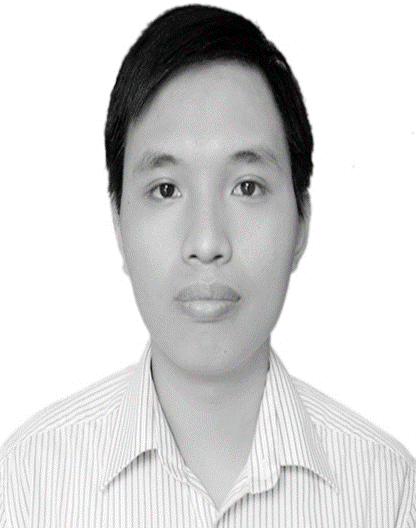
\includegraphics[width=1in,height=1.25in,clip,keepaspectratio]{lac.png}}]{Lac Van Duong} 
was born in Vietnam, in February 1991. He received the Engineering  degree (with the excellent degree) in Mechatronics from Hanoi University of Science and Technology (HUST), in 2014, and the M.S. degree in 2016. He is now a PhD student at Japan Advanced Institutes of Science and Technology (JAIST). His research interests include the applications of Control Systems, Robotics, and Mechatronics. He is recipient of 2014 Honda Young Engineer and Scientist’s Award.
\end{IEEEbiography}
\vskip -3\baselineskip plus -1fil
\begin{IEEEbiography}[{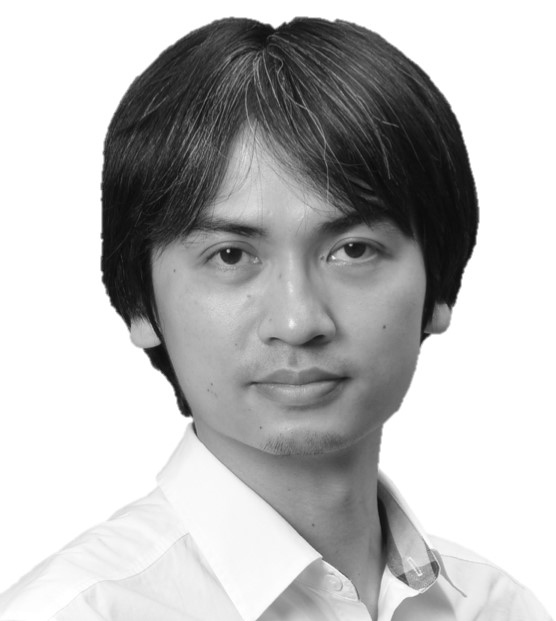
\includegraphics[width=1in,height=1.25in,clip,keepaspectratio]{van.jpg}}]{Van Anh Ho} 
obtained the PhD degree on Robotics at Ritsumeikan Unviersity, Japan in 2012. He had completed the JSPS Post doctoral fellow in 2013 before joining Advanced Research Center Mitsubishi Electric Corp. in Japan. From 2015 to 2017 he worked as Assistant Professor at Ryukoku University in Kyoto where he led a laboratory on soft haptics. From 2017 he joined Japan Advanced Institute of Science and Technology (JAIST) for setting up a laboratory on Soft Robotics. His curent research interests are soft robotics, soft haptic interaction, tactile sensing, grasping and manipulation, bio-inspired robots. He is recipient of 2019 IEEE Nagoya Chapter Young Researcher Award, Best Paper Finalists at IEEE SII (2016) and IEEE RoboSoft (2020). He is member of IEEE, RSJ.
\end{IEEEbiography}
% if you will not have a photo at all:
%\begin{IEEEbiographynophoto}{John Doe}
%Biography text here.
%\end{IEEEbiographynophoto}
% insert where needed to balance the two columns on the last page with
% biographies
%\newpage
% You can push biographies down or up by placing
% a \vfill before or after them. The appropriate
% use of \vfill depends on what kind of text is
% on the last page and whether or not the columns
% are being equalized.
\vfill
% Can be used to pull up biographies so that the bottom of the last one
% is flush with the other column.
%\enlargethispage{-5in}
% that's all folks
\end{document}


